\subsection{INNER AUTOMORPHISMS}

Let \(G\) be a group. The set \(\operatorname{Aut}(G)\) of automorphisms of the group \(G\) is a subgroup of \(\mathfrak{S}_{\mathbb{G}}\) (§ 4, no. 1, Example 2).

PROPOSITION 3. Let G be a group. For every element x of G, the mapping \(\operatorname{Int}(x): y \mapsto xyx^{-1}\) of G into itself is an automorphism of G. The mapping \(\operatorname{Int}: x \mapsto \operatorname{Int}(x)\) of G into \(\operatorname{Aut}(G)\) is a group homomorphism, whose kernel is the centre of G and whose image is a normal subgroup of \(\operatorname{Aut}(G)\) .

If x, y and z are elements of G, then \((xyx^{-1})(xzx^{-1}) = xyzx^{-1}\) and hence \(\operatorname{Int}(x)\) is an endomorphism of G. For x and y elements of G,

\[
\operatorname{Int} (x) \circ \operatorname{Int} (y) = \operatorname{Int} (x y):
\]

for all \(z \in G\) , \(x(yzy^{-1})x^{-1} = (xy)z(xy)^{-1}\) . On the other hand, \(\operatorname{Int}(e)\) is the identity mapping of G. The mapping Int is therefore a monoid homomorphism from G to the monoid \(\operatorname{End}(G)\) of endomorphisms of the group G. As the elements of G are invertible, the mapping Int takes its values in the set \(\operatorname{Aut}(G)\) of invertible elements of \(\operatorname{End}(G)\) (§ 2, no. 3). Now \(xyx^{-1} = y\) if and only if x and y commute and hence \(\operatorname{Int}(x)\) is the identity mapping of G if and only if x is a central element. Finally, let \(\alpha\) be an automorphism of G and let \(x \in G\) ; then

\[
\operatorname{Int} (\alpha (x)) = \alpha \circ \operatorname{Int} (x) \circ \alpha^ {- 1}.\tag{2}
\]

For \(y \in G\) ,

\[
\alpha (x). y. \alpha (x) ^ {- 1} = \alpha (x). \alpha (\alpha^ {- 1} (y)). \alpha (x) ^ {- 1} = \alpha (x. \alpha^ {- 1} (y). x ^ {- 1}).
\]

Hence \(\alpha\) . Int(G). \(\alpha^{-1} \subset \operatorname{Int}(G)\) .

DEFINITION 4. Let G be a group and \(x \in \mathbf{G}\) . The automorphism \(y \mapsto xyx^{-1}\) is called the inner automorphism of G defined by \(x\) and is denoted by Int \(x\) .

For \(x, y \in G\) , we also write \(x^y = y^{-1}xy = (\operatorname{Int} y^{-1})(x)\) .

A subgroup of G is normal if and only if it is stable under all inner automorphisms of G (§ 4, no. 4, Definition 5). A subgroup of G is called characteristic if it stable under all automorphisms of G. The centre of a group G is a characteristic subgroup (formula (2)).

The centre of a group G is not necessarily stable under all endomorphisms of G (Exercise 22). In particular, the centre of a group with operators is not necessarily a stable subgroup.

PROPOSITION 4. Let G be a group, H a characteristic (resp. normal) subgroup of G and K a characteristic subgroup of H. Then K is a characteristic (resp. normal) subgroup of G.

The restriction to H of an automorphism (resp. inner automorphism) of G is an automorphism of H and therefore leaves K invariant.

Let G be a group, A ⊂ G and \(b \in G\) . b is said to normalize A if \(bAb^{-1} = A\) ; b is said to centralize A if, for all \(a \in A\) , \(bab^{-1} = a\) . Let A and B be subsets of G; B is said to normalize (resp. centralize) A if every element of B normalizes (resp. centralizes) A.

The set of \(g \in G\) which normalize (resp. centralize) A is called the normalizer (resp. centralizer) of A (cf.~§1, no. 5, Definition 9); it is often denoted by \(N_{G}(A)\) or simply \(N(A)\) (resp. \(C_{G}(A)\) or \(C(A)\) ). It is a subgroup of G. When A is a subgroup of G, \(N_{G}(A)\) may be characterized as the largest subgroup of G which contains A and in which A is normal.

Remarks. (1) The normalizer (resp. centralizer) of A is the strict stabilizer (resp. fixer) of A when G operates on itself by inner automorphisms. In particular the centralizer is a normal subgroup of the normalizer.

\begin{enumerate}
\def\labelenumi{(\arabic{enumi})}
\setcounter{enumi}{1}
\tightlist
\item
  The set of elements \(b \in \mathbf{G}\) such that \(b\mathbf{A}b^{-1} \subset \mathbf{A}\) is a submonoid of \(\mathbf{G}\) . Even when \(\mathbf{A}\) is a subgroup of \(\mathbf{G}\) , this set is not necessarily a subgroup of \(\mathbf{G}\) (Exercise 27).
\end{enumerate}

\subsection{ORBITS}

DEFINITION 5. Let G be a group, E a G-set and \(x \in G\) . An element \(y \in E\) is conjugate to x under the operation of G if there exists an element \(\alpha \in G\) such that \(y = \alpha x\) . The set of conjugate elements of x is called the orbit of x in E.

The relation ``y is conjugate to x'' is an equivalence relation. For x = ex; if \(y = \alpha x\) , then \(x = \alpha^{-1} y\) ; if \(y = \alpha x\) and \(z = \beta y\) , then \(z = \beta \alpha x\) . The orbits are the equivalence classes under this relation.

A subset X of E is stable if and only if it is saturated with respect to the relation of conjugation.

The mapping \(\alpha\mapsto\alpha x\) of G into E is sometimes called the orbital mapping defined by x. It is a G-morphism of G (with the operation of G on itself by left translation) into E. The image G.x of G under this mapping is the orbit of x.

G is said to operate freely on E if, for all \(x \in E\) , the orbital mapping defined by x is injective or also if the mapping \((g, x) \mapsto (gx, x)\) of G × E into E × E is injective.

Examples. (1) Let G be a group and consider the operation of G on itself by inner automorphisms. Two elements of G which are conjugate under this operation are called conjugate under inner automorphisms or simply conjugate. The orbits are called conjugacy classes. Similarly, two subsets H and \(H'\) of G are called conjugate if there exists an element \(\alpha \in G\) such that \(H' = \alpha \cdot H \cdot \alpha^{-1}\) , that is if they are conjugate under the extension to \(\mathfrak{P}(G)\) of the operation of G on itself by inner automorphisms.

\begin{enumerate}
\def\labelenumi{(\arabic{enumi})}
\setcounter{enumi}{1}
\tightlist
\item
  *In the space \(\mathbf{R}^n\) , the orbit of a point \(x\) under the action of the orthogonal group \(\mathbf{O}(n, \mathbf{R})\) is the Euclidean sphere of radius \(\| x \|\) .
\end{enumerate}

The stabilizers of two conjugate elements of E are conjugate subgroups of G (no. 2, Proposition 2).

The quotient set of E under the relation of conjugation is the set of orbits of E; it is sometimes denoted by E/G or \(G\backslash E\). (Sometimes the notation E/G is reserved for the case where E is a right G-set and the notation \(G\backslash E\) for the case where E is a left G-set.)

Let G be a group operating on a set E on the right. Let H be a normal subgroup of G. The group G operates on E/H on the right, the corresponding law of right action being \((xH, g) \mapsto xHg = xgH\) ; under this operation, H operates trivially, whence a right operation of G/H on E/H. Let \(\phi\) be the canonical mapping of E/H onto E/G; the inverse images under \(\phi\) of the points of E/G are the orbits of G (or of G/H) in E/H. Hence \(\phi\) defines when passing to the quotient a bijection, called canonical, of \((\mathrm{E}/\mathrm{H})/\mathrm{G} = (\mathrm{E}/\mathrm{H})/(\mathrm{G}/\mathrm{H})\) onto E/G.

Let G (resp. H) be a group operating on a set E on the left (resp. right). Suppose that the actions of G and H on E commute, that is

\[
(g. x). h = g. (x. h) \quad \text { for } g \in \mathrm{G}, x \in \mathrm{E} \text { and } h \in \mathrm{H}.
\]

The action of H on E is also a left operation of the opposite group \(H^{0}\) to H. It then follows from § 4, no. 9, Proposition 12 that the mapping which associates with the element \((g, h) \in G \times H^{0}\) the mapping \(x \mapsto g \cdot x \cdot h\) of E into itself is a left operation of \(G \times H^{0}\) on E. The orbit of an element \(x \in E\) under this operation is the set GxH. The set of these orbits is denoted by \(G\backslash E/H\). On the other hand, the operation of G (resp. H) is compatible with the relation of conjugation with respect to the operation of H (resp. G) and the set of orbits \(G\backslash(E/H)\) (resp. \((G\backslash E)/H\)) is identified with \(G\backslash E/H\): in the diagram

\pandocbounded{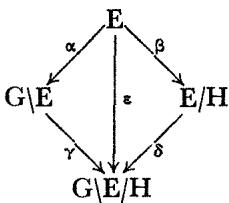
\includegraphics[keepaspectratio]{images/part001_b92675b5.jpg}}

(where \(\alpha, \beta, \gamma, \delta, \varepsilon\) denote the canonical mappings of taking quotients), \(\gamma \circ \alpha = \delta \circ \beta = \varepsilon\) .

Let G be a group and H a subgroup of G. Consider the right operation of H on G by right translation (no. 1, Example 2). The set of orbits G/H is the set of left cosets modulo H; note that G operates on G/H on the left by the law \((g, xH) \mapsto gxH\) (cf.~no. 5). Similarly, the set of right cosets modulo H is the set \(H\backslash G\) of orbits of the left operation of H on G by left translation. If K is a subgroup of G containing H and \(\Gamma\) is a left (resp. right) coset modulo H, then \(\Gamma K\) (resp. \(K\Gamma\) ) is a left (resp. right) coset modulo K. The mapping \(\Gamma \mapsto \Gamma K\) (resp. \(\Gamma \mapsto K\Gamma\) ) is called the canonical mapping of G/H into G/K (resp. of \(H\backslash G\) into \(K\backslash G\)). It is surjective.

Let G be a group and H and K two subgroups of G. Let H operate on G on the left by left translation and K on the right by right translation; these two operations commute, which allows us to consider the set \(H\backslash G/K\). The elements of \(H\backslash G/K\) are called the double cosets of G modulo H and K. When K = H, we simply say double cosets modulo H. For the canonical mapping of G/H onto \(H\backslash G/H\) to be a bijection, it is necessary and sufficient that H be a normal subgroup of G.

\subsection{HOMOGENEOUS SETS}

DEFINITION 6. Let G be a group. An operation of G on a set E is called transitive if there exists an element \(x \in E\) whose orbit is E. A G-set E is called homogeneous if the operation of G on E is transitive.

It is also said that G operates transitively on E; or that E is a homogeneous set under G. It amounts to the same to say that E is non-empty and that, for all elements x and y of E, there exists an element \(\alpha \in G\) such that \(\alpha.x = y\) .

Example. If E is a G-set, each orbit of E, with the induced operation, is a homogeneous set under G.

Let G be a group and H a subgroup of G. Consider the set G/H of left cosets modulo H. The group G operates on G/H on the left by \((g, xH) \mapsto gxH\) . Let N be the normalizer of H. The group N operates on G/H on the right by \((xH, n) \mapsto xHn = xnH\) . This operation induces on H the trivial operation and hence, on passing to the quotient, N/H operates on G/H on the right. Let \(\phi: (N/H)^{0} \to S_{G/H}\) be the homomorphism corresponding to this operation.

PROPOSITION 5. With the above notation, G/H is a homogeneous G-set. The mapping \(\phi\) induces an isomorphism of \((\mathrm{N} / \mathrm{H})^0\) onto the group of automorphisms of the G-set G/H.

The orbit in G/H of the element \(\dot{e}=H\) is G/H, whence the first assertion. We now prove the second. If \(n\in N\) defines by right translation the identity mapping on G/H, then \(\dot{e}.n=\dot{e}\) , that is H.n=H, whence \(n\in H\) . Therefore

N/H operates faithfully on G/H on the right and \(\phi\) is injective. The left operation of G and right operation of N/H on G/H commute and hence the operators of N/H define G-morphisms of G/H into itself, which are necessarily G-automorphisms since they are bijective. Therefore \(\phi\) takes its values in the group \(\Phi\) of G-automorphisms of G/H. We show that the image of \(\phi\) is \(\Phi\) . Let \(f \in \Phi\) . By transporting the structure, the stabilizer of \(f(\dot{e})\) in G is equal to the stabilizer of \(\dot{e}\) and hence to H. Let \(n \in G\) be such that \(f(\dot{e}) = n\dot{e}\) . The stabilizer of \(n\dot{e}\) in G is \(nHn^{-1}\) (no. 2, Proposition 2), whence \(nHn^{-1} = H\) and \(n \in N\) . For every element xH of G/H, \(f(xH) = f(x.\dot{e}) = x.f(\dot{e}) = xnH = xHn\) and f coincides with the mapping defined by n.

Remarks. (1) Let G be a group, H a subgroup of G and \(\phi: \mathbf{G} \to \mathfrak{S}_{\mathbf{G}/\mathbf{H}}\) the homomorphism corresponding to the operation of G on G/H. The kernel of \(\phi\) is the intersection of the conjugates of H (no. 2, Proposition 2). It is also the largest normal subgroup contained in H (no. 3). In particular, G operates faithfully on G/H if and only if the intersection of the conjugates of H reduces to \(\{e\}\) .

\begin{enumerate}
\def\labelenumi{(\arabic{enumi})}
\setcounter{enumi}{1}
\tightlist
\item
  Let G be a group and H and K subgroups such that H is a normal subgroup of K. Then K/H operates on the G-set G/H on the right and the canonical mapping of G/H onto G/K defines on passing to the quotient a G-set isomorphism \((G/H)/(K/H) \rightarrow G/K\) (cf.~no. 4).
\end{enumerate}

PROPOSITION 6. Let G be a group, E a homogeneous G-set, \(a \in E\) , H the stabilizer of \(a\) and K a subgroup of G contained in H. There exists one and only one G-morphism \(f\) of G/K into E such that \(f(e.K) = a\) . If K = H, \(f\) is an isomorphism.

If \(f\) is a solution, then \(f(x, \mathbf{K}) = x.a\) for all \(x\) in \(\mathbf{G}\) , whence the uniqueness; we show the existence. The orbital mapping defined by \(a\) is compatible with the equivalence relation \(y \in x\mathbf{K}\) on \(\mathbf{G}\) . For, if \(y = xk, k \in \mathbf{K}\) , then

\[
y. a = x k. a = x. a.
\]

A mapping \(f\) is thus derived of \(G / K\) into \(H\) which satisfies \(f(x, \mathbf{K}) = x.a\) for all \(x\) in \(G\) . This mapping is a G-morphism and \(f(\mathbf{K}) = a\) . This mapping is surjective for its image is a non-empty stable subset of \(E\) . Suppose now that \(K = H\) and let us show that \(f\) is injective. If \(f(x, \mathbf{H}) = f(y, \mathbf{H})\) , then \(x.a = y.a\) , whence \(x^{-1}y.a = a\) and \(x^{-1}y \in H\) , whence \(x.H = y.H\) .

THEOREM 1. Let G be a group.

\begin{enumerate}
\def\labelenumi{(\alph{enumi})}
\item
  Every homogeneous G-set is isomorphic to a homogeneous G-set of the form G/H where H is a subgroup of G.
\item
  Let H and H' be two subgroups of G. The G-sets G/H and G/H' are isomorphic if and only if H and H' are conjugate.
\end{enumerate}

As a homogeneous G-set is non-empty, assertion (a) follows from Proposition 6. We show (b). Let \(f: \mathrm{G} / \mathrm{H} \to \mathrm{G} / \mathrm{H}'\) be a G-set isomorphism. The subgroup H is the stabilizer of H and hence, by transport of structure, the stabilizer of an element of G/H'. The subgroups H and H' are therefore conjugate (no. 2, Proposition 2). If H' = αHα⁻¹, H' is the stabilizer of the element α. H of G/H (no. 2, Proposition 2) and hence G/H' is isomorphic to G/H (Proposition 6).

Examples. (1) Let E be a non-empty set. The group \(S_{E}\) operates transitively on E. If x and y are two elements of E, the mapping \(\tau: E \to E\) such that \(\tau(x) = y\) , \(\tau(y) = x\) and \(\tau(z) = z\) for \(z \neq x\) , y, is a permutation of E. Let \(a \in E\) . The stabilizer of a is identified with \(S_{F}\) , where \(F = E - \{a\}\) . The homogeneous G-set E is thus isomorphic to \(S_{E}/S_{F}\) .

\begin{enumerate}
\def\labelenumi{(\arabic{enumi})}
\setcounter{enumi}{1}
\tightlist
\item
  Let \(\mathbf{E}\) be a set of \(n\) elements and \((p_i)_{i\in \mathbf{I}}\) a finite family of integers \(>0\) such that \(\sum_{i}p_{i} = n\) . Let \(\mathbf{X}\) be the set of partitions \((\mathrm{F}_i)_{i\in \mathbf{I}}\) of \(\mathbf{E}\) such that \(\operatorname {Card}(\mathrm{F}_i) = p_i\) for all \(i\) . The group \(\mathfrak{S}_{\mathbf{E}}\) operates transitively on \(\mathbf{X}\) . The stabilizer H of an element \((\mathrm{F}_i)_{i\in \mathbf{I}}\) of \(\mathbf{X}\) is canonically isomorphic to \(\prod_{i\in \mathbf{I}}\mathfrak{S}_{\mathbf{F}_i}\) and is hence of order \(\prod_{i\in \mathbf{I}}p_i!\) . Applying Theorem 1 and §4, no. 4, Corollary to Proposition 4, a new proof is obtained of the fact that
\end{enumerate}

\[
\operatorname{Card} (\mathbf {X}) = \frac {n !}{\prod_ {i \in I} p _ {i} !}.
\]

In particular, take \(\mathbf{I} = \{1,2,\dots,r\}\) , \(\mathbf{E} = \{1,2,\dots,n\}\) ,

\[
\mathrm{F} _ {i} = \left\{p _ {1} + \dots + p _ {i - 1} + 1, \dots , p _ {1} + \dots + p _ {i} \right\}
\]

for \(1 \leqslant i \leqslant r\) . Let \(S\) be the set of \(\tau \in \mathfrak{S}_{E}\) such that \(\tau|_{F_i}\) is increasing for \(1 \leqslant i \leqslant r\) . If \((G_1, \ldots, G_r) \in X\) there exists one and only one \(\tau \in S\) which maps \((F_1, \ldots, F_r)\) to \((G_1, \ldots, G_r)\) . In other words, each left coset of \(\mathfrak{S}_{E}\) modulo \(H\) meets \(S\) in one and only one point.

\begin{enumerate}
\def\labelenumi{(\arabic{enumi})}
\setcounter{enumi}{2}
\tightlist
\item
  *Let \(n\) be an integer \(\geqslant 1\) . The orthogonal group \(\mathbf{O}(n, \mathbf{R})\) operates transitively on the unit sphere \(\mathbf{S}_{n-1}\) in \(\mathbf{R}^n\) . The stabilizer of the point \((0, \ldots, 0, 1)\) is identified with the orthogonal group \(\mathbf{O}(n-1, \mathbf{R})\) . The homogeneous \(\mathbf{O}(n, \mathbf{R})\) -set \(\mathbf{S}_{n-1}\) is thus isomorphic to \(\mathbf{O}(n, \mathbf{R}) / \mathbf{O}(n-1, \mathbf{R})\) .*
\end{enumerate}

\subsection{HOMOGENEOUS PRINCIPAL SETS}

DEFINITION 7. Let G be a group. An operation of G on a set E is called simply transitive if there exists an element x of E such that the orbital mapping defined by x is a bijection. A set E, together with a simply transitive left action of G on E, is called a left homogeneous principal G-set (or left homogeneous principal set under G).

It amounts to the same to say that G operates freely and transitively on E, or also that there exists an element \(x \in E\) such that the orbital mapping defined by x is an isomorphism of the G-set G (where G operates by left translation) onto E; or also that the two following conditions are satisfied:

\begin{enumerate}
\def\labelenumi{(\roman{enumi})}
\item
  E is non-empty.
\item
  for all elements \(x\) and \(y\) of \(\mathbf{E}\) , there exists one and only one element \(\alpha \in \mathbf{G}\) such that \(\alpha x = y\) .
\end{enumerate}

Condition (ii) is also equivalent to the following condition:

\begin{enumerate}
\def\labelenumi{(\roman{enumi})}
\setcounter{enumi}{2}
\tightlist
\item
  the mapping \((\alpha, x) \mapsto (\alpha x, x)\) is a bijection of \(G \times E\) onto \(E \times E\) .
\end{enumerate}

We leave to the reader the task of defining right homogeneous principal G-sets.

Examples. (1) Let G operate on itself by left (resp. right) translation. Thus a left (resp. right) homogeneous principal G-set structure is defined on G, which is sometimes denoted by \(G_{s}\) (resp. \(G_{d}\) ).

\begin{enumerate}
\def\labelenumi{(\arabic{enumi})}
\setcounter{enumi}{1}
\item
  Let E be a homogeneous set under a commutative group G. If G operates faithfully on E, the latter is a homogeneous principal G-set.
\item
  Let E and F be two isomorphic sets with structures of the same species and let \(\operatorname{Isom}(\mathbf{E}, \mathbf{F})\) be the set of isomorphisms of E onto F (with the given structures). The group \(\operatorname{Aut}(\mathbf{E})\) of automorphisms of E (with the given structure) operates on \(\operatorname{Isom}(\mathbf{E}, \mathbf{F})\) on the right by the law \((\sigma, f) \mapsto f \circ \sigma\) and \(\operatorname{Isom}(\mathbf{E}, \mathbf{F})\) is a right homogeneous principal \(\operatorname{Aut}(\mathbf{E})\) -set. Similarly, the group \(\operatorname{Aut}(\mathbf{F})\) operates on \(\operatorname{Isom}(\mathbf{E}, \mathbf{F})\) on the left by the law \((\sigma, f) \mapsto \sigma \circ f\) and \(\operatorname{Isom}(\mathbf{E}, \mathbf{F})\) is a left homogeneous principal \(\operatorname{Aut}(\mathbf{F})\) -set.
\item
  *A homogeneous principal set under the additive group of a vector space is called an affine space (cf.~II, § 9, no. 1).*
\end{enumerate}

The group of automorphisms of the homogeneous principal G-set \(G_{s}\) (Example 1) is the group of right translations of G which is identified with \(G^{0}\) (no. 5, Proposition 5). Let E be a homogeneous principal G-set and a an element of E. The orbital mapping \(\omega_{a}\) defined by a is an isomorphism of the G-set \(G_{s}\) onto E. By transporting the structure an isomorphism \(\psi_{a}\) is derived of \(G^{0}\) onto Aut(E). It should be noted that \(\psi_{a}\) in general depends on a; more precisely, for \(\alpha \in G\) ,

\[
\psi_ {\alpha a} = \psi_ {a} \circ \operatorname{Int} _ {\mathbf {G} ^ {0}} (\alpha) = \psi_ {a} \circ \operatorname{Int} (\alpha^ {- 1}).\tag{3}
\]

For, writing \(\delta_{a}\) for the translation \(x\mapsto x\alpha\) on G,

\[
\omega_ {\alpha a} = \omega_ {a} \circ \delta_ {\alpha}
\]

and

\[
\psi_ {a} (x) = \omega_ {a} \circ \delta_ {x} \circ \omega_ {a} ^ {- 1}, \quad x \in G,
\]

whence

\[
\psi_ {\alpha a} (x) = \omega_ {a} \circ \delta_ {\alpha} \circ \delta_ {x} \circ \delta_ {\alpha} ^ {- 1} \circ \omega_ {a} ^ {- 1} = \omega_ {a} \circ \delta_ {\alpha^ {- 1} x \alpha} \circ \omega_ {a} ^ {- 1} = \psi_ {a} (\alpha^ {- 1} x \alpha).
\]

\subsection{PERMUTATION GROUPS OF A FINITE SET}

If E is a finite set with n elements, the symmetric group \(S_{E}\) (§ 4, no. 1) is a finite group of order \(n!\) . When E is the interval \([1, n]\) of the set N of natural numbers, the corresponding symmetric group is denoted by \(S_{n}\) ; the symmetric group of any set with n elements is isomorphic to \(S_{n}\) .

DEFINITION 8. Let E be a finite set, \(\zeta \in \mathfrak{S}_{\mathrm{E}}\) a permutation of E and \(\bar{\zeta}\) the subgroup of \(\mathfrak{S}_{\mathrm{E}}\) generated by \(\zeta\) . \(\zeta\) is called a cycle if, under the operation of \(\bar{\zeta}\) on E, there exists one and only one orbit which is not reduced to a single element. This orbit is called the support of \(\zeta\) .

Let \(\zeta\) be a cycle. The support \(\operatorname{supp}(\zeta)\) of \(\zeta\) is the set of \(x \in E\) such that \(\zeta(x) \neq x\) .

The order of a cycle \(\zeta\) is equal to the cardinal of its support. The subgroup \(\bar{\zeta}\) generated by \(\zeta\) operates transitively and faithfully on \(\operatorname{supp}(\zeta)\) . As \(\zeta\) is commutative, \(\operatorname{supp}(\zeta)\) is a principal set under \(\bar{\zeta}\) (no. 6, Example 2) and hence \(\operatorname{Card}(\operatorname{supp}(\zeta)) = \operatorname{Card}(\bar{\zeta})\) .

Lemma 1. Let \((\zeta_{i})_{i\in I}\) be a family of cycles whose supports are pairwise disjoint. Then the \(\zeta_{i}\) are pairwise permutable. Let \(\sigma = \prod_{i\in I}\zeta_{i}\) and \(\overline{\sigma}\) be the subgroup generated by \(\sigma\) . Then \(\sigma(x) = \zeta_{i}(x)\) for \(x\in S_{i}, i\in I\) , and \(\sigma(x) = x\) for \(x\notin \bigcup_{i\in I}S_{i}\) . The mapping \(i\mapsto S_i\) is a bijection of I onto the set of \(\overline{\sigma}\) -orbits not consisting of a single element.

Let \(\zeta\) and \(\zeta'\) be two cycles whose supports are disjoint. If

\[
x \notin \operatorname{supp} (\zeta) \cup \operatorname{supp} \left(\zeta^ {\prime}\right),
\]

then \(\zeta\zeta'(x) = \zeta'\zeta(x) = x\) . If \(x\) belongs to the support of \(\zeta\) , then \(\zeta'(x) = x\) and \(\zeta(x)\) belongs to the support of \(\zeta\) , whence \(\zeta\zeta'(x) = \zeta'\zeta(x) = \zeta(x)\) . Similarly when \(x\) belongs to the support of \(\zeta'\) , then \(\zeta'\zeta(x) = \zeta\zeta'(x) = \zeta'(x)\) . Hence \(\zeta\zeta' = \zeta'\zeta\) . Therefore the \(\zeta_i\) are pairwise permutable and, for \(i \in I\) and \(x \in S_i\) , \(\sigma(x) = \zeta_i(x) \in S_i\) . The mappings \(\sigma\) and \(\zeta_i\) coincide on \(S_i\) , hence \(S_i\) is stable under \(\sigma\) and the subgroup of \(\mathfrak{S}_{S_i}\) generated by the restriction of \(\sigma\) to \(S_i\) operates transitively on \(S_i\) ; therefore \(S_i\) is a \(\overline{\sigma}\) -orbit. As the \(S_i\) are non-empty and are pairwise disjoint, the mapping \(i \mapsto S_i\) is injective. As \(\bigcup_{i} S_i\) is the set of \(x\) such that \(\sigma(x) \neq x\) , every \(\overline{\sigma}\) -orbit not consisting of a single element is one of the \(S_i\) .

PROPOSITION 7. Let E be a finite set and \(\sigma\) a permutation of E. There exists one and only one finite set C of cycles satisfying the two following conditions:

\begin{enumerate}
\def\labelenumi{(\alph{enumi})}
\item
  the supports of the elements of C are pairwise disjoints;
\item
  \(\sigma = \prod_{\zeta \in C} \zeta\) (the elements of \(C\) being pairwise permutable by Lemma 1). Let \(\bar{\sigma}\) be the subgroup generated by \(\sigma\) and let \(S\) be the set of \(\bar{\sigma}\) -orbits not consisting of a single element. For \(s \in S\) , write \(\zeta_s(x) = \sigma(x)\) if \(x \in s\) and \(\zeta_s(x) = x\) if \(x \notin s\) . For all \(s \in S\) , \(\zeta_s\) is a cycle whose support is \(s\) and \(\sigma = \prod_{s \in S} \zeta_s\) , as is seen by applying the two sides to any element of \(E\) . The uniqueness of \(C\) follows from Lemma 1.
\end{enumerate}

DEFINITION 9. A cycle of order 2 is called a transposition.

Let \(x\) and \(y\) be two distinct elements of \(E\) . Let \(\tau_{x,y}\) denote the unique transposition with support \(\{x, y\}\) .

For every permutation \(\sigma\) of E the permutation \(\sigma. \tau_{x,y}. \sigma^{-1}\) is a transposition whose support is \(\{\sigma(x), \sigma(y)\}\) . Hence:

\[
\sigma . \tau_ {x, y}. \sigma^ {- 1} = \tau_ {\sigma (x), \sigma (y)}.\tag{4}
\]

Transpositions thus form a conjugacy class in the group \(\mathfrak{S}_{\mathbb{E}}\) .

PROPOSITION 8. Let E be a finite set. The group \(\mathfrak{S}_{\mathrm{E}}\) is generated by the transpositions.

For every permutation \(\sigma\) let \(F_{\sigma}\) be the set of \(x \in E\) such that \(\sigma(x) = x\) . We show by descending induction on \(p\) that every permutation \(\sigma\) such that \(\operatorname{Card}(F_{\sigma}) = p\) is a product of transpositions. If \(p \geqslant \operatorname{Card}(E)\) , the permutation \(\sigma\) is the identity mapping of \(E\) ; it is the product of the empty family of transpositions. If \(p < \operatorname{Card}(E)\) , suppose that the property is proved for every permutation \(\sigma'\) such that \(\operatorname{Card}(F_{\sigma'}) > p\) . Now \(E - F_{\sigma} \neq \varnothing\) ; let \(x \in E - F_{\sigma}\) and \(y \in \sigma(x)\) . Then \(y \neq x\) and \(y \in E - F_{\sigma}\) . Let \(\sigma' = \tau_{x,y} \cdot \sigma\) . The set \(F_{\sigma'}\) contains \(F_{\sigma}\) and \(x\) and hence \(\operatorname{Card}(F_{\sigma'}) > \operatorname{Card}(F_{\sigma}) = p\) . By the induction hypothesis \(\sigma'\) is a product of transpositions and hence \(\sigma = \tau_{x,y} \cdot \sigma'\) is a product of transpositions.

PROPOSITION 9. Let \(n\) be an integer \(\geqslant 0\) . The group \(\mathfrak{S}_n\) is generated by the transpositions \((\tau_{i,i+1})_{1\leqslant i\leqslant n-1}\) .

By virtue of Proposition 8, it suffices to show that every transposition \(\tau_{p,q}\) , \(1 \leqslant p < q \leqslant n\) , belongs to the subgroup H generated by the \(\tau_{i,i+1}\) , \(1 \leqslant i \leqslant n-1\) . We show this by induction on \(q-p\) . For \(q-p=1\) , it is obvious. If \(q-p>1\) , then (formula (4)) \(\tau_{p,q} = \tau_{q-1,q}\tau_{p,q-1}\tau_{q-1,q}\) . By the induction hypothesis \(\tau_{p,q-1} \in H\) and therefore \(\tau_{p,q} \in H\) .

If \(\sigma \in \mathfrak{S}_n\) , every ordered pair \((i,j)\) of elements of \([1,n]\) such that \(i < j\) and \(\sigma(i) > \sigma(j)\) is called an inversion of \(\sigma\) . Let \(\nu(\sigma)\) denote the number of inversions of \(\sigma\) .

Let P be the additive group of mappings from \(Z^{n}\) to Z. For \(f \in P\) and \(\sigma \in S_{n}\) , let \(\sigma f\) be the element of P defined by

\[
\sigma f (z _ {1}, \dots , z _ {n}) = f (z _ {\sigma (1)}, \dots , z _ {\sigma (n)}).\tag{5}
\]

The action of \(\mathfrak{S}_n\) on \(\mathbf{P}\) thus defined is an operation; for all \(\sigma, \tau \in \mathfrak{S}_n\) and \(f \in \mathbf{P}, ef = f\) and

\[
\begin{array}{r l} \left(\tau (\sigma f)\right) (z _ {1}, \dots , z _ {n}) & = \sigma f (z _ {\tau (1)}, \dots , z _ {\tau (n)}) = f (z _ {\tau \sigma (1)}, \dots , z _ {\tau \sigma (n)}) \\ & = ((\tau \sigma) f) (z _ {1}, \dots , z _ {n}). \end{array}
\]

Formula (5) shows that \(\sigma(-f) = -\sigma f\) for \(\sigma \in \mathfrak{S}_n\) and \(f \in P\) .

Let \(p\) be the element of P defined by

\[
p (z _ {1}, \dots , z _ {n}) = \prod_ {i <   j} (z _ {j} - z _ {i}).\tag{6}
\]

Lemma 2. \(p \neq 0\) and \(\sigma p = (-1)^{\nu(\sigma)}\) for \(\sigma \in \mathfrak{S}_n\) .

\(p(1,2,\ldots,n) = \prod_{i < j}(j - i)\neq 0\) and hence \(p\neq 0\) . On the other hand, if \(\sigma \in \mathfrak{S}_n\) , then

\[
\sigma p (z _ {1}, \dots , z _ {n}) = p (z _ {\sigma (1)}, \dots , z _ {\sigma (n)}) = \prod_ {i <   j} (z _ {\sigma (j)} - z _ {\sigma (i)}).
\]

Let C be the set of ordered pairs \((i,j)\) such that \(1 \leqslant i \leqslant n\) , \(1 \leqslant j \leqslant n\) , i \textless{} j. A permutation \(\theta\) is defined on C by setting \(\theta(i,j) = (\sigma(i), \sigma(j))\) if \((i,j)\) is not an inversion, \(\theta(i,j) = (\sigma(j), \sigma(i))\) if \((i,j)\) is an inversion. This implies \(\sigma p = (-1)^{\nu(\sigma)} p\) .

THEOREM 2. Let E be a finite set. There exists one and only one homomorphism \(\varepsilon\) from \(\mathfrak{S}_n\) to the multiplicative group \(\{-1, +1\}\) such that \(\varepsilon(\tau) = -1\) for every transposition \(\tau\) .

The uniqueness follows from Proposition 8. We show the existence. By transporting the structure, it may be assumed that \(\mathbf{E} = [1, n]\) . Using the above notation, let \(\varepsilon(\sigma) = (-1)^{\nu(\sigma)}\) . Then (Lemma 2)

\[
\sigma (\sigma^ {\prime} p) = \sigma (\varepsilon (\sigma^ {\prime}) p) = \varepsilon (\sigma^ {\prime}) (\sigma p) = \varepsilon (\sigma^ {\prime}) \varepsilon (\sigma) p.
\]

On the other hand,

\[
\sigma (\sigma^ {\prime} p) = (\sigma \sigma^ {\prime}) p = \varepsilon (\sigma \sigma^ {\prime}) p.
\]

As \(p \neq -p\) , it follows that \(\varepsilon(\sigma\sigma') = \varepsilon(\sigma)\varepsilon(\sigma')\) and thus \(\varepsilon\) is a homomorphism. We now show that, for every transposition \(\tau, \varepsilon(\tau) = -1\) . \(\nu(\tau_{n-1,n}) = 1\) , whence \(\varepsilon(\tau_{n-1,n}) = -1\) . As every transposition \(\tau\) is conjugate to \(\tau_{n-1,n}\) and the group \(\{-1, +1\}\) is commutative, \(\varepsilon(\tau) = \varepsilon(\tau_{n-1,n}) = -1\) .

DEFINITION 10. In the notation of Theorem 2, the number \(\varepsilon(\sigma)\) (also denoted \(\varepsilon_{\sigma}\) ) is called the signature of the permutation \(\sigma\) . The kernel of the homomorphism \(\varepsilon\) is called the alternating group of E.

\(\sigma\) is called even (resp. odd) if \(\varepsilon(\sigma) = 1\) (resp. \(\varepsilon(\sigma) = -1\) ). The alternating group of E is denoted by \(\mathfrak{A}_{\mathbb{E}}\) . It is a normal subgroup of \(\mathfrak{S}_{\mathbb{E}}\) . When \(\mathbf{E} = [1, n]\) , it is simply denoted by \(\mathfrak{A}_{n}\) . When the cardinal \(n\) of E is \(\geqslant 2\) , it is a subgroup of index 2 and hence of order \(n! / 2\) . It can be shown that, for \(n = 3\) or \(n \geqslant 5\) , the group \(\mathfrak{A}_{n}\) is a simple group (cf.~Exercise 16).

Example. If \(\sigma\) is a cycle of order \(d\) , then

\[
\varepsilon (\sigma) = (- 1) ^ {d - 1}.
\]

The number of inversions of the permutation

\[
(1, 2, 3, \dots , d) \mapsto (d, 1, 2, \dots , d - 1)
\]

is equal to \(d - 1\) .

\section{EXTENSIONS, SOLVABLE GROUPS, NILPOTENT GROUPS}

Throughout this paragraph, the group laws are, unless expressly mentioned otherwise, written multiplicatively.

\subsection{EXTENSIONS}

DEFINITION 1. Let F and G be two groups. An extension of G by F is a triple \(\mathcal{E} = (\mathrm{E}, i, p)\) , where E is a group, \(i\) an injective homomorphism of F into E and \(p\) a surjective homomorphism of E onto G such that \(\operatorname{Im}(i) = \operatorname{Ker}(p)\) . A homomorphism \(s: \mathrm{G} \to \mathrm{E}\) (resp. \(r: \mathrm{E} \to \mathrm{F}\) ) such that \(p \circ s = \operatorname{Id}_{\mathbf{G}}\) (resp. \(r \circ i = \operatorname{Id}_{\mathbf{F}}\) ) is called a section (resp. retraction) of the extension \(\mathcal{E}\) .

An extension \(\mathcal{E} = (\mathrm{E}, i, p)\) of \(\mathbf{G}\) by \(\mathbf{F}\) is often denoted by the diagram \(\mathcal{E}: \mathrm{F} \xrightarrow{i} \mathrm{E} \xrightarrow{p} \mathrm{G}\) , in which \(i\) and \(p\) are sometimes omitted if no confusion can arise. It is sometimes said simply that the group \(\mathbf{E}\) is an extension of \(\mathbf{G}\) by \(\mathbf{F}\) .

For a group E to be an extension of G by F, it is necessary and sufficient that it contain a normal subgroup \(F'\) isomorphic to F such that the quotient group \(E/F'\) is isomorphic to G.

An extension \(\mathcal{E}\colon\mathrm{F}\xrightarrow{i}\mathrm{E}\xrightarrow{p}\mathrm{G}\) is called central if the image \(i(\mathrm{F})\) is contained in the centre of E; this is only possible if F is commutative.

Let \(\mathcal{E}:\mathrm{F}\xrightarrow{i}\mathrm{E}\xrightarrow{p}\mathrm{G}\) and \(\mathcal{E}':\mathrm{F}\xrightarrow{i'}\mathrm{E}'\xrightarrow{p'}\mathrm{G}\) be two extensions of G by F. A morphism of \(\mathcal{E}\) into \(\mathcal{E}'\) is a homomorphism \(u:\mathrm{E}\to\mathrm{E}'\) such that \(p'\circ u=p\) and \(u\circ i=i'\) , or, in other words, such that the following diagram is commutative:

\pandocbounded{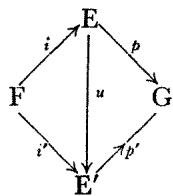
\includegraphics[keepaspectratio]{images/part001_e41623d9.jpg}}

PROPOSITION 1. Let \(\mathcal{E}: F \xrightarrow{i} E \xrightarrow{p} G\) and \(\mathcal{E}': F \xrightarrow{i'} E' \xrightarrow{p'} G\) be extensions of \(G\) by \(F\) . If \(u: E \to E'\) is a morphism of \(\mathcal{E}\) into \(\mathcal{E}'\) , \(u\) is an isomorphism of \(E\) onto \(E'\) and \(u^{-1}\) is a morphism of \(\mathcal{E}'\) into \(\mathcal{E}\) .

Let \(x \in E\) be such that \(u(x) = e\) . Then \(p(x) = p'(u(x)) = e\) , whence \(x \in i(F)\) . Let \(y \in F\) be such that \(x = i(y)\) ; then \(i'(y) = u(i(y)) = e\) . As \(i'\) is injective, \(y = e\) and \(x = e\) . Therefore \(u\) is injective. By virtue of §4, no. 6, Corollary 1 to Proposition 7, \(u\) is surjective since \(u(i(F)) = i'(F)\) . The last assertion is immediate.

In other words, the extensions \(\mathcal{E}\) and \(\mathcal{E}'\) are isomorphic if and only if there exists a morphism of \(\mathcal{E}\) into \(\mathcal{E}'\) .

Let \(\mathbf{F}\) and \(\mathbf{G}\) be two groups and write \(\mathbf{E}_0 = \mathbf{F} \times \mathbf{G}\) ; let \(i: \mathbf{F} \to \mathbf{E}_0\) be the canonical injection and \(p: \mathbf{E}_0 \to \mathbf{G}\) be the canonical projection. Every extension of \(\mathbf{G}\) by \(\mathbf{F}\) isomorphic to the extension \(\mathcal{E}_0: \mathbf{F} \xrightarrow{i} \mathbf{E}_0 \xrightarrow{p} \mathbf{G}\) is called a trivial extension.

PROPOSITION 2. Let \(\mathcal{E}:\mathrm{F}\xrightarrow{i}\mathrm{E}\xrightarrow{p}\mathrm{G}\) be an extension of \(\mathrm{G}\) by \(\mathrm{F}\) . The following conditions are equivalent:

\begin{enumerate}
\def\labelenumi{(\roman{enumi})}
\item
  \(\mathcal{E}\) is a trivial extension;
\item
  \(\mathcal{E}\) has a retraction \(r\) ;
\item
  \(\mathcal{E}\) has a section \(s\) such that \(s(\mathbf{G})\) is contained in the centralizer of \(i(\mathbf{F})\) .
\end{enumerate}

Clearly (i) implies (ii) and (iii). If (ii) holds, the mapping \((r, p): \mathbf{E} \to \mathbf{F} \times \mathbf{G}\) is a morphism of \(\mathcal{E}\) into \(\mathcal{E}_0\) , whence (i). If (iii) holds, the homomorphism of \(\mathbf{F} \times \mathbf{G}\) into \(\mathbf{E}\) corresponding to \((i, s)\) ( \(\S 4\) , no. 9, Proposition 12) is a morphism of \(\mathcal{E}_0\) into \(\mathcal{E}\) , whence (i).

It may be that an extension \(\mathcal{E}:\mathbf{F}\to\mathbf{E}\to\mathbf{G}\) is not trivial and yet the group \(\mathbf{E}\) is isomorphic to \(\mathbf{F}\times\mathbf{G}\) (Exercise 6).

DEFINITION 2. Let F and G be two groups and \(\tau\) a homomorphism of G into the automorphism group of F. Write \(\tau(g)(f) = {}^g f\) for \(g \in G\) and \(f \in F\) . The set \(\mathbf{F} \times \mathbf{G}\) with the law of composition

\[
((f, g), (f ^ {\prime}, g ^ {\prime})) \mapsto (f, g) \cdot_ {\tau} (f ^ {\prime}, g ^ {\prime}) = (f. ^ {g} f ^ {\prime}, g g ^ {\prime})\tag{1}
\]

is called the external semi-direct product of G by F relative to \(\tau\) .

The external semi-direct product of G by F relative to \(\tau\) is denoted by \(F \times_{\tau} G\) .

PROPOSITION 3. The external semi-direct product \(\mathbf{F} \times_{\tau} \mathbf{G}\) is a group. The mappings \(i: \mathbf{F} \to \mathbf{F} \times_{\tau} \mathbf{G}\) defined by \(i(f) = (f, e)\) , \(p: \mathbf{F} \times_{\tau} \mathbf{G} \to \mathbf{G}\) defined by \(p(f, g) = g\) , and \(s: \mathbf{G} \to \mathbf{F} \times_{\tau} \mathbf{G}\) defined by \(s(g) = (e, g)\) are group homomorphisms. The triple \((\mathbf{F} \times_{\tau} \mathbf{G}, i, p)\) is an extension of \(\mathbf{G}\) by \(\mathbf{F}\) and \(s\) is a section of the extension.

We have:

\[
\begin{array}{r l} ((f, g) \cdot_ {\tau} (f ^ {\prime}, g ^ {\prime})) \cdot_ {\tau} (f ^ {\prime \prime}, g ^ {\prime \prime}) & = (f. ^ {g} f ^ {\prime}, g g ^ {\prime}) \cdot_ {\tau} (f ^ {\prime \prime}, g ^ {\prime \prime}) \\ & = (f. ^ {g} f ^ {\prime}. ^ {g g ^ {\prime}} f ^ {\prime \prime}, g g ^ {\prime} g ^ {\prime \prime}); \\ (f, g) \cdot_ {\tau} ((f ^ {\prime}, g ^ {\prime}) \cdot_ {\tau} (f ^ {\prime \prime}, g ^ {\prime \prime})) & = (f, g) \cdot_ {\tau} (f ^ {\prime}. ^ {g ^ {\prime}} f ^ {\prime \prime}, g ^ {\prime} g ^ {\prime \prime}) \\ & = (f. ^ {g} (f ^ {\prime}. ^ {g ^ {\prime}} f ^ {\prime \prime}), g g ^ {\prime} g ^ {\prime \prime}). \end{array}
\]

Now \({}^{g}(f'.{}^{g'}f'') = {}^{g}f'.{}^{gg'}f''\) , which shows that the law of composition defined by (1) is associative. The element \((e, e)\) is the identity under this law. The element \((f, g)\) admits as inverse \((^{g^{-1}}f^{-1}, g^{-1})\) . Hence the law of composition on \(F \times_{\tau} G\) is a group law. The other assertions are immediate.

Using the notation of Proposition 3, \(E_{\tau}\) will denote the extension

\[
\mathrm{F} \xrightarrow {i} \mathrm{F} \times_ {\tau} \mathrm{G} \xrightarrow {p} \mathrm{G}.
\]

Let \(\mathcal{E}'\colon F\stackrel{i'}{\to}E'\stackrel{p'}{\to}G\) be an extension of \(G\) by \(F\) and \(s'\colon G\to E'\) a section of \(\mathcal{E}'\) . We define an operation \(\tau\) of \(G\) on the group \(F\) by:

\[
i ^ {\prime} (\tau (g, f)) = s ^ {\prime} (g) i ^ {\prime} (f) s ^ {\prime} (g) ^ {- 1} = \operatorname{Int} (s ^ {\prime} (g)) (i ^ {\prime} (f)).\tag{2}
\]

PROPOSITION 4. With the above notation, there exists one and only one isomorphism \(u\) of \(\mathcal{E}_{\tau}\) onto \(\mathcal{E}'\) such that \(u \circ s = s'\) .

\((f, g) = (f, e) \cdot_ {\tau} (e, g) = i(f).s(g)\) . Therefore, if u is a solution to the problem, of necessity \(u(f,g)=i'(f).s'(g)\) , whence the uniqueness of u. We prove the existence. We write \(u(f,g)=i'(f).s'(g)\) . Then

\[
\begin{array}{r l} u (f, g) \cdot u (f ^ {\prime}, g ^ {\prime}) & = i ^ {\prime} (f) s ^ {\prime} (g) i ^ {\prime} (f ^ {\prime}) s ^ {\prime} (g ^ {\prime}) \\ & = i ^ {\prime} (f) (s ^ {\prime} (g) i ^ {\prime} (f ^ {\prime}) s ^ {\prime} (g) ^ {- 1}) s ^ {\prime} (g) s ^ {\prime} (g ^ {\prime}) \\ & = i ^ {\prime} (f) i ^ {\prime} (\tau (g, f ^ {\prime})) \cdot s ^ {\prime} (g) s ^ {\prime} (g ^ {\prime}) \\ & = i ^ {\prime} (f \cdot \tau (g, f ^ {\prime})) \cdot s ^ {\prime} (g g ^ {\prime}) \\ & = u ((f, g) \cdot_ {\tau} (f ^ {\prime}, g ^ {\prime})). \end{array}
\]

Therefore, \(u\) is a homomorphism of \(\mathbf{F} \times_{\tau} \mathbf{G}\) into \(\mathbf{E}'\) . Obviously \(u \circ i = i'\) , \(p' \circ u = p\) and \(u \circ s = s'\) .

Remark. The definition of the operation \(\tau\) by formula (2) depends on the extension \(\mathcal{E}'\) and the section \(s'\) . When F is commutative, the operation \(\tau\) does not depend on \(s'\) . For \(\operatorname{Int}(s'(g)) \mid i'(F)\) depends then only on the coset of \(s'(g)\) mod. \(i'(F)\) .

More generally, let \(\mathcal{E}:\mathrm{F}\to \mathrm{E}\to \mathrm{G}\) be an extension of \(\mathbf{G}\) by a commutative group \(\mathbf{F}\) (it is not assumed that \(\mathcal{E}\) admits a section). The group \(\mathbf{E}\) operates on \(\mathbf{F}\) by inner automorphisms, this image is trivial on the image of \(\mathbf{F}\) and hence defines an operation of \(\mathbf{G}\) on \(\mathbf{F}\) . If \(\mathcal{E}\) admits a section, this operation is that defined by formula (2).

COROLLARY. Let G be a group and H and K two subgroups of G such that H is normal, \(\mathbf{H} \cap \mathbf{K} = \{e\}\) and \(\mathbf{H} \cdot \mathbf{K} = \mathbf{G}\) . Let \(\tau\) be the operation of \(\mathbf{K}\) on \(\mathbf{H}\) by inner automorphisms of \(\mathbf{G}\) . The mapping \((h, k) \mapsto hk\) is an isomorphism of \(\mathbf{H} \times_{\tau} \mathbf{K}\) onto \(\mathbf{G}\) .

Under the hypotheses of this corollary, G is said to be the semi-direct product of K by H.

Examples. (1) Let G be a group and E a homogeneous principal G-set; let \(\Gamma\) denote the automorphism group of G. Let A be the set of permutations f of E with the following property:

There exists \(\gamma \in \Gamma\) such that \(f\) is a \(\gamma\) -morphism of \(\mathbf{E}\) into \(\mathbf{E}\) (that is, \(f(gb) = \gamma(g)f(b)\) for \(b \in \mathbf{E}\) and \(g \in \mathbf{G}\) ).

The above formula \(f(gb) = \gamma(g)f(b)\) shows that if \(f \in A\) there exists a unique \(\gamma \in \Gamma\) such that \(f\) is a \(\gamma\) -morphism, we shall denote it by \(p(f)\) .

Let \(f, f'\) be in A, \(\gamma = p(f), \gamma' = p(f')\) . Then, for all \(b \in E\) and all \(g \in G\) ,

\[
(f ^ {\prime} \circ f) (g b) = f ^ {\prime} (\gamma (g) f (b)) = \gamma^ {\prime} (\gamma (g)) f ^ {\prime} (f (b))
\]

which proves that \(f' \circ f \in \mathbf{A}\) and that \(p(f' \circ f) = p(f')p(f)\) . On the other hand, \(f(\gamma^{-1}(g)f^{-1}(b)) = gb\) , whence \(f^{-1}(gb) = \gamma^{-1}(g)f^{-1}(b)\) and \(f^{-1} \in \mathbf{A}\) . Thus \(\mathbf{A}\) is a subgroup of \(\mathfrak{S}_{\mathbf{E}}\) and \(p\) is a homomorphism of \(\mathbf{A}\) into \(\Gamma\) . The kernel of \(p\) is the set \(\operatorname{Aut}_{\mathbf{G}}(\mathbf{E})\) of automorphisms of the \(\mathbf{G}\) -set \(\mathbf{E}\) .

We fix \(a \in \mathbf{E}\) . We have defined in § 5, no. 6 an isomorphism \(\psi_a\) of \(\mathbf{G}^0\) onto \(\operatorname{Aut}_{\mathbf{G}}(\mathbf{E})\) such that \(\psi_a(x)(ga) = gxa\) for all \(g, x\) in \(\mathbf{G}\) . On the other hand, for \(\gamma \in \Gamma\) , let \(s_a(\gamma)\) be the permutation of \(\mathbf{E}\) defined by \(s_a(\gamma)(ga) = \gamma(g)a\) for all \(g \in \mathbf{G}\) ; it is immediately verified that \(s_a\) is a homomorphism of \(\Gamma\) into \(\mathbf{A}\) such that \(p \circ s_a = \operatorname{Id}_{\Gamma}\) . Thus \(\mathbf{G}^0 \xrightarrow{\psi_a} \mathbf{A} \xrightarrow{p} \Gamma\) is an extension of \(\Gamma\) by \(\mathbf{G}^0\) and \(s_a\) is a section of this extension. This extension and this section define an operation of \(\Gamma\) on \(\mathbf{G}^0\) , \(s_a(\Gamma)\) acting on \(\psi_a(\mathbf{G}^0)\) by inner automorphisms; we write this operation exponentially. We show that this operation is the natural operation (§ 3, no. 1, Example 3): for \(x, g\) in \(\mathbf{G}\) and \(\gamma \in \Gamma\) ,

\[
\begin{array}{r l} (\psi_ {a} (^ {\gamma} x)) (g a) & = (s _ {a} (\gamma) \circ \psi_ {a} (x) \circ s _ {a} (\gamma) ^ {- 1}) (g a) \\ & = (s _ {a} (\gamma) \circ \psi_ {a} (x)) (\gamma^ {- 1} (g) a) = s _ {a} (\gamma) (\gamma^ {- 1} (g) x a) \\ & = g \gamma (x) a = \psi_ {a} (\gamma (x)) g a \end{array}
\]

whence \({}^{\gamma}x = \gamma(x)\) .

Proposition 4 then shows that A is isomorphic to the semidirect product of \(\Gamma = \operatorname{Aut}(\mathbf{G})\) by \(\mathbf{G}^0\) under the natural operation of \(\operatorname{Aut}(\mathbf{G})\) on \(\mathbf{G}^0\) . Note that the isomorphism which we have constructed depends in general on the choice of the element \(a \in \mathbf{E}\) .

\begin{enumerate}
\def\labelenumi{(\arabic{enumi})}
\setcounter{enumi}{1}
\tightlist
\item
  *Let A be a commutative ring. The upper triangular group T(n, A) is the semi-direct product of the diagonal subgroup D(n, A) by the upper strict triangular group T1(n, A).*
\end{enumerate}

\subsection{COMMUTATORS}

DEFINITION 3. Let G be a group and x and y two elements of G. The element \(x^{-1}y^{-1}xy\) of G is called the commutator of x and y.

\((x,y)\) is used to denote the commutator of x and y. Then obviously

\[
(y, x) = (x, y) ^ {- 1}.
\]

For \(x\) and \(y\) to commute it is necessary and sufficient that \((x, y) = e\) . More generally,

\[
x y = y x (x, y).
\]

On the other hand we write

\[
x ^ {y} = y ^ {- 1} x y = x (x, y) = (y, x ^ {- 1}) x.\tag{3}
\]

As the mapping \(x \mapsto x^y\) is the inner automorphism \(\operatorname{Int}(y^{-1})\) , \((x, y)^z = (x^z, y^z)\) for all \(x, y, z \in G\) .

For \(x, y, z \in G\) , we prove the following relations:

\[
(x, y z) = (x, z). (x, y) ^ {z} = (x, z). (z, (y, x)). (x, y)\tag{4}
\]

(4 bis) \((xy,z) = (x,z)^y.(y,z) = (x,z).(((x,z),y).(y,z))\)

\begin{enumerate}
\def\labelenumi{(\arabic{enumi})}
\setcounter{enumi}{4}
\item
  \((x^{y}, (y, z)).(y^{z}, (z, x)).(z^{x}, (x, y)) = e\)
\item
  \((x, yz).(z, xy).(y, zx) = e\)
\end{enumerate}

(6 bis) \((xy, z). (yz, x). (zx, y) = e.\)

Now

\[
\begin{array}{r l} (x, y z) & = x ^ {- 1} z ^ {- 1} y ^ {- 1} x y z = (x, z) z ^ {- 1} x ^ {- 1} y ^ {- 1} x y z = (x, z) (x, y) ^ {z} \\ & = (x, z) (z, (x, y) ^ {- 1}) (x, y) \end{array}
\]

by (3), which proves (4). Formula (4 bis) follows similarly. On the other hand,

\[
\begin{array}{r l} (x ^ {y}, (y, z)) & = (x ^ {y}) ^ {- 1} (z, y) (x ^ {y}) (y, z) \\ & = y ^ {- 1} x ^ {- 1} y z ^ {- 1} y ^ {- 1} z y y ^ {- 1} x y y ^ {- 1} z ^ {- 1} y z \\ & = (y z y ^ {- 1} x y) ^ {- 1} (z x z ^ {- 1} y z). \end{array}
\]

Then writing \(u = yzy^{-1}xy\) , \(v = zxz^{-1}yz\) and \(w = xyx^{-1}zx\) , we obtain

\[
(x ^ {y}, (y, z)) = u ^ {- 1} v.
\]

By cyclically permuting \(x, y, z\) , we deduce \((y^z, (z, x)) = v^{-1}w\) and

\[
\left(z ^ {x}, (x, y)\right) = w ^ {- 1} u,
\]

which immediately imply (5). Finally, (6) follows by multiplying together the two sides in the three formulae obtained by cyclically permuting x, y, z in the formula \((x, yz) = x^{-1}z^{-1}y^{-1}xyz = (yzx)^{-1}(xyz)\) , and similarly for (6 bis).

If A and B are two subgroups of G, (A, B) denotes the subgroup generated by the commutators \((a, b)\) with \(a \in A\) and \(b \in B\) . Then \((A, B) = \{e\}\) if and only if A centralizes B. \((A, B) \subset A\) if and only if B normalizes A. If A and B are normal (resp. characteristic), so is \((A, B)\) .

PROPOSITION 5. Let A, B, C be three subgroups of G.

\begin{enumerate}
\def\labelenumi{(\roman{enumi})}
\item
  The subgroup A normalizes the subgroup (A, B).
\item
  If the subgroup (B, C) normalizes A, the subgroup (A, (B, C)) is generated by the elements \((a, (b, c))\) with \(a \in \mathbf{A}\) , \(b \in \mathbf{B}\) and \(c \in \mathbf{C}\) .
\item
  If A, B and C are normal, then
\end{enumerate}

\[
(\mathrm{A}, (\mathrm{B}, \mathrm{C})) \subset (\mathrm{C}, (\mathrm{B}, \mathrm{A})). (\mathrm{B}, (\mathrm{C}, \mathrm{A})).
\]

By (4 bis), for \(a, a' \in \mathbf{A}\) and \(b \in \mathbf{B}\) ,

\[
(a, b) ^ {a ^ {\prime}} = (a a ^ {\prime}, b). (a ^ {\prime}, b) ^ {- 1},
\]

whence (i). Suppose now that (B, C) normalizes A. For \(a \in \mathbf{A}\) , \(b \in \mathbf{B}\) , \(c \in \mathbf{C}\) and \(x \in \mathbf{G}\) , (4) implies

\[
(a, (b, c). x) = (a, x). (x, ((b, c), a)) (a, (b, c))
\]

and \(((b, c), a) \in \mathbf{A}\) since (B, C) normalizes A, whence by induction on \(p\) the fact that \(\left(a, \prod_{i=1}^{p} (b_i, c_i)\right)\) , for \(b_i \in \mathbf{B}\) , \(c_i \in \mathbf{C}\) , belongs to the subgroup generated by the elements of the form \((a, (b, c))\) . If finally A, B and C are normal, so are the subgroups (A, (B, C)), (C, (B, A)) and (B, (C, A)). It therefore suffices by (ii) to show that

\[
(a, (b, c)) \in (\mathrm{C}, (\mathrm{B}, \mathrm{A})). (\mathrm{B}, (\mathrm{C}, \mathrm{A}))
\]

for all \(a \in \mathbf{A}\) , \(b \in \mathbf{B}\) and \(c \in \mathbf{C}\) . Now by (5), writing \(a^{b^{-1}} = u\)

\[
(a, (b, c)) = ((u ^ {b}), (b, c)) = (c ^ {u}, (u, b)) ^ {- 1}. (b ^ {c}, (c, u)) ^ {- 1},
\]

whence (iii).

DEFINITION 4. Let G be a group. The subgroup generated by the commutators of elements of G is called the derived group of G.

The derived group of G is thus the subgroup (G, G). It is also denoted by D(G). By an abuse of language, it is sometimes called the commutator group of G although it is in general distinct from the set of commutators of elements of G (Exercise 16). D(G) = \{e\} if and only if G is commutative.

PROPOSITION 6. Let \(f: \mathbf{G} \to \mathbf{G}'\) be a group homomorphism. Then \(f(\mathbf{D}(\mathbf{G})) \subset \mathbf{D}(\mathbf{G}')\) . If \(f\) is surjective, the homomorphism of \(\mathbf{D}(\mathbf{G})\) into \(\mathbf{D}(\mathbf{G}')\) the restriction of \(f\) is surjective.

The image under \(f\) of a commutator of elements of \(G\) is a commutator of elements of \(G'\) . If \(f\) is surjective, the image under \(f\) of the set of commutators of \(G\) is the set of commutators of \(G'\) . The proposition thus follows from § 4, no. 3, Corollary 3 to Proposition 2.

COROLLARY 1. The derived group of a group G is a characteristic subgroup of G. In particular it is a normal subgroup of G.

COROLLARY 2. Let G be a group. The quotient group G/D(G) is commutative. Let \(\pi: G \to G/D(G)\) be the canonical homomorphism. Every homomorphism \(f\) of G into a commutative group \(G'\) can be expressed uniquely in the form \(f = \bar{f} \circ \pi\) , where \(\bar{f}: G/D(G) \to G'\) is a homomorphism.

Now \(\pi (\mathbf{D}(\mathbf{G})) = \{e\}\) . As \(\pi\) is surjective, it follows that \(\mathbf{D}(\mathbf{G} / \mathbf{D}(\mathbf{G})) = \{e\}\) , whence the first assertion. The second follows from § 4, no. 4, Proposition 5.

COROLLARY 3. Let H be a subgroup of G. The following conditions are equivalent:

\begin{enumerate}
\def\labelenumi{(\roman{enumi})}
\item
  \(\mathbf{H} \supset \mathbf{D}(\mathbf{G})\) ;
\item
  H is a normal subgroup and G/H is commutative.
\item
  (ii) \(\Rightarrow\) (i) by Corollary 2 and (i) \(\Rightarrow\) (ii) by §4, no. 7, Theorem 4, since every subgroup of a commutative group is normal.
\end{enumerate}

COROLLARY 4. Let G be a group and X a subset of G which generates G. The group D(G) is the normal subgroup of G generated by the commutators of elements of X.

Let H be the normal subgroup of G generated by the commutators of elements of X and \(\phi: G \to G/H\) the canonical homomorphism. The set \(\phi(X)\) generates G/H. The elements of \(\phi(X)\) are pairwise permutable and hence H is commutative ( \(\S 4\) , no. 3, Corollary 2 to Proposition 2). Hence (Corollary 3) H contains D(G). On the other hand, obviously \(H \subset D(G)\) .

Remarks. (1) Corollary 2 can also be expressed by saying that G/D(G), together with \(\pi\) , is a solution of the universal mapping problem for G, relative to commutative groups and homomorphisms from G to commutative groups.

\begin{enumerate}
\def\labelenumi{(\arabic{enumi})}
\setcounter{enumi}{1}
\tightlist
\item
  Under the hypotheses of Corollary 4, the subgroup generated by the commutators of elements of X is contained in D(G) but is not in general equal to D(G) (cf.~Exercise 15e).
\end{enumerate}

Examples. (1) If \(\mathbf{G}\) is a non-commutative simple group, then \(\mathrm{D}(\mathbf{G}) = \mathbf{G}\) . Therefore every homomorphism of \(\mathbf{G}\) into a commutative group is trivial.

\begin{enumerate}
\def\labelenumi{(\arabic{enumi})}
\setcounter{enumi}{1}
\tightlist
\item
  The derived group of the symmetric group \(\mathfrak{S}_n\) is the alternating group \(\mathfrak{A}_n\) . For \(\mathfrak{A}_n\) is generated by the products of two transpositions; if \(\tau = \tau_{x,y}\) and \(\tau' = \tau_{x',y'}\) are two transpositions, let \(\sigma\) be a permutation such that \(\sigma(x') = x\) and \(\sigma(y') = y\) . Then \(\tau' = \sigma^{-1}\tau\sigma\) and \(\tau\tau' = \tau^{-1}\tau' = \tau^{-1}\sigma^{-1}\tau\sigma\) is a commutator. Hence \(\mathfrak{A}_n \subset D(\mathfrak{S}_n)\) . As \(\mathfrak{S}_n / \mathfrak{A}_n\) is commutative, \(\mathfrak{A}_n \supset D(\mathfrak{S}_n)\) (Corollary 3).
\end{enumerate}

\subsection{LOWER CENTRAL SERIES, NILPOTENT GROUPS}

Let \(\mathbf{G}\) be a group, \(\mathbf{H}\) a subgroup of \(\mathbf{G}\) and \(\mathbf{K}\) a normal subgroup of \(\mathbf{G}\) . The image of \(\mathbf{H}\) in \(\mathbf{G} / \mathbf{K}\) is contained in the centre of \(\mathbf{G} / \mathbf{K}\) if and only if \((\mathbf{G}, \mathbf{H}) \subset \mathbf{K}\) .

DEFINITION 5. Let G be a group. The lower central series of G is the sequence \((\mathbf{C}^n (\mathbf{G}))_{n\geqslant 1}\) of subgroups of G defined inductively by:

\[
\mathbf {C} ^ {1} (\mathbf {G}) = \mathbf {G}, \quad \mathbf {C} ^ {n + 1} (\mathbf {G}) = (\mathbf {G}, \mathbf {C} ^ {n} (\mathbf {G})).
\]

Let \(f: \mathbf{G} \to \mathbf{G}'\) be a group homomorphism. It is seen, by induction on \(n\) , that \(f(\mathbf{C}^n(\mathbf{G})) \subset \mathbf{C}^n(\mathbf{G}')\) and that, if \(f\) is surjective, \(f(\mathbf{C}^n(\mathbf{G})) = \mathbf{C}^n(\mathbf{G}')\) . In particular, for all \(n \geqslant 1\) , \(\mathbf{C}^2(\mathbf{G})\) is a characteristic (and hence normal) subgroup of \(\mathbf{G}\) . For all \(n \geqslant 1\) , \(\mathbf{C}^n(\mathbf{G}) / \mathbf{C}^{n+1}(\mathbf{G})\) is contained in the centre of \(\mathbf{G} / \mathbf{C}^{n+1}(\mathbf{G})\) .

Let \((\mathbf{G}_1, \mathbf{G}_2, \ldots)\) be a decreasing sequence of normal subgroups of \(\mathbf{G}\) such that (1) \(\mathbf{G}_1 = \mathbf{G}\) ; (2) for all \(i\) , \(\mathbf{G}_i / \mathbf{G}_{i+1}\) is contained in the centre of \(\mathbf{G} / \mathbf{G}_{i+1}\) . Then \(\mathbf{C}^i(\mathbf{G}) \subset \mathbf{G}_i\) , as is seen by induction on \(i\) .

Now

\[
\left(\mathbf {C} ^ {m} (\mathbf {G}), \mathbf {C} ^ {n} (\mathbf {G})\right) \subset \mathbf {C} ^ {m + n} (\mathbf {G}).\tag{7}
\]

For, if this relation is denoted by \((\mathbf{F}_{m,n})\) , it follows from \((\mathbf{F}_{m,n})\) , by no. 2, Proposition 5, that

\[
\begin{array}{l} \left(\mathrm{C} ^ {m} (\mathrm{G}), \mathrm{C} ^ {n + 1} (\mathrm{G})\right) \subset \left(\mathrm{G}, \left(\mathrm{C} ^ {m} (\mathrm{G}), \mathrm{C} ^ {n} (\mathrm{G})\right)\right). \left(\mathrm{C} ^ {n} (\mathrm{G}), \left(\mathrm{G}, \mathrm{C} ^ {m} (\mathrm{G})\right)\right) \\ \subset \mathrm{C} ^ {m + n + 1} (\mathrm{G}). \left(\mathrm{C} ^ {m + 1} (\mathrm{G}), \mathrm{C} ^ {n} (\mathrm{G})\right). \end{array}
\]

Hence \(((\mathbf{F}_{m,n})\) and \((\mathbf{F}_{m + 1,n}))\Rightarrow (\mathbf{F}_{m,n + 1})\) . As \((\mathbf{F}_{m,1})\) and \((\mathbf{F}_{1,n})\) are obvious \((\mathbf{F}_{m,n})\) follows by induction.

DEFINITION 6. A group G is called nilpotent if there exists an integer n such that \(\mathbf{C}^{n+1}(\mathbf{G}) = \{e\}\) . The least integer n such that \(\mathbf{C}^{n+1}(\mathbf{G}) = \{e\}\) is called the nilpotency class of a nilpotent group G.

If \(n \in N\) , a group of nilpotency class n is called a nilpotent group of class n.~It is sometimes said that the nilpotency class of a group G is finite if G is nilpotent.

Examples. (1) A group is nilpotent of class 0 (resp. \(\leqslant 1\) ) if and only if it consists of the identity element (resp. is commutative).

\begin{enumerate}
\def\labelenumi{(\arabic{enumi})}
\setcounter{enumi}{1}
\item
  *For every commutative ring A and every integer \(n \geqslant 1\) , the upper strict triangular group \(\mathrm{T}_1(n, \mathbf{A})\) is nilpotent of class \(\leqslant n - 1\) (and exactly of class \(n - 1\) if \(\mathbf{A} \neq \{0\}\) ).*
\item
  Let \(\mathbf{G}\) be a nilpotent group of class \(n\) . Every subgroup (resp. every quotient group) of \(\mathbf{G}\) is nilpotent of class \(\leqslant n\) . For, if \(\mathbf{H}\) is a subgroup of \(\mathbf{G}\) , then \(\mathbf{C}^n (\mathbf{H})\subset \mathbf{C}^n (\mathbf{G})\) . If \(\mathbf{G}'\) is a quotient group of \(\mathbf{G}\) and \(\pi : \mathbf{G}\to \mathbf{G}'\) is the canonical homomorphism, then \(\mathbf{C}^n (\mathbf{G}') = \pi (\mathbf{C}^n (\mathbf{G}))\) .
\item
  A finite product of nilpotent groups is nilpotent.
\end{enumerate}

PROPOSITION 7. Let G be a group and n an integer. The following conditions are equivalent:

\begin{enumerate}
\def\labelenumi{(\alph{enumi})}
\item
  G is nilpotent of class \(\leqslant n\) .
\item
  There exists a series of subgroups of \(\mathbf{G}\) :
\end{enumerate}

\[
\mathrm{G} = \mathrm{G} ^ {1} \supset \mathrm{G} ^ {2} \supset \dots \supset \mathrm{G} ^ {n + 1} = \{e \}
\]

such that \((\mathbf{G},\mathbf{G}^k)\subset \mathbf{G}^{k + 1}\) for all \(k\in [1,n]\) .

\begin{enumerate}
\def\labelenumi{(\alph{enumi})}
\setcounter{enumi}{2}
\item
  There exists a subgroup \(\mathbf{A}\) of \(\mathbf{G}\) contained in the centre of \(\mathbf{G}\) such that \(\mathbf{G} / \mathbf{A}\) is nilpotent of class \(\leqslant n - 1\) .
\item
  (a) \(\Rightarrow\) (b): it suffices to take \(\mathbf{G}^k = \mathbf{C}^k (\mathbf{G})\) .
\item
  (b) \(\Rightarrow\) (a): by induction on \(k\) , \(\mathbf{C}^k (\mathbf{G})\subset \mathbf{G}^k\)
\item
  (a) \(\Rightarrow\) (c): it suffices to take \(\mathbf{A} = \mathbf{C}^n (\mathbf{G})\) .
\item
  (c) \(\Rightarrow\) (a): let \(\pi: \mathbf{G} \to \mathbf{G} / \mathbf{A}\) be the canonical homomorphism; then \(\pi(\mathbf{C}^n(\mathbf{G})) = \mathbf{C}^n(\mathbf{G} / \mathbf{A}) = \{e\}\) and hence \(\mathbf{C}^n(\mathbf{G}) \subset \mathbf{A}\) , whence \(\mathbf{C}^{n+1}(\mathbf{G}) = \{e\}\) .
\end{enumerate}

More briefly: a group is nilpotent of class \(\leqslant n\) if it can be obtained from the group \(\{e\}\) by n successive central extensions.

COROLLARY. A central extension of a nilpotent group (by a necessarily commutative group) is nilpotent.

PROPOSITION 8. Let G be a nilpotent group of class \(\leqslant n\) and let H be a subgroup of G. There exists a sequence of subgroups

\[
\mathbf {G} = \mathbf {H} ^ {1} \supset \mathbf {H} ^ {2} \supset \dots \supset \mathbf {H} ^ {n + 1} = \mathbf {H},
\]

such that \(\mathbf{H}^{k + 1}\) is normal in \(\mathbf{H}^k\) and \(\mathbf{H}^k /\mathbf{H}^{k + 1}\) is commutative for all \(k\leqslant n\)

Choose a sequence \((\mathbf{G}^{k})\) of subgroups of G satisfying the conditions of Proposition 7 (b) for all k; \(G^{k}\) is normal in G. Write:

\[
\mathbf {H} ^ {k} = \mathbf {H}. \mathbf {G} ^ {k}.
\]

It is necessary to verify that \(\mathbf{H}^{k + 1}\) is normalized by \(\mathbf{H}^k = \mathbf{H}.\mathbf{G}^k\) ; as it is normalized by \(\mathbf{H}\) , it suffices to verify that it is by \(\mathbf{G}^k\) . Now, if \(s\in \mathbf{G}^k\) and \(h\in \mathbf{H}\) ,

\[
s h s ^ {- 1} = s h s ^ {- 1} h ^ {- 1}. h \in (\mathrm{G}, \mathrm{G} ^ {k}). \mathrm{H}
\]

and \((\mathbf{G},\mathbf{G}^k)\) . H is contained in \(\mathbf{G}^{k + 1}\) . \(\mathbf{H} = \mathbf{H}^{k + 1}\) ; hence \(s.\mathbf{H}^{k + 1}.s^{-1} = \mathbf{H}^{k + 1}\) , which shows that \(\mathbf{H}^{k + 1}\) is normal in \(\mathbf{H}^k\) .

Finally, the canonical homomorphism \(G^{k}/G^{k+1} \to H^{k}/H^{k+1}\) is obviously surjective; as the first group is commutative, so is the second.

COROLLARY 1. Let G be a nilpotent group and H a subgroup of G. If H is distinct from G, the normalizer \(N_{G}(H)\) of H in G is distinct from H.

Let \(k\) be the largest index such that \(H^{k} \neq H\) . The group \(H^{k}\) normalizes \(H\) and is distinct from \(H\) .

COROLLARY 2. Let G be a nilpotent group and H a subgroup of G. If H is distinct from G, there exists a normal subgroup N of G, containing H, distinct from G and such that G/N is commutative.

Let \(k\) be the least index such that \(H^k \neq G\) . The group \(H^k\) satisfies the required conditions.

COROLLARY 3. Let G be a nilpotent group and H a subgroup of G. If G = H.(G, G), then G = H.

Every subgroup N of G which contains H and such that G/N is commutative contains H.(G, G). Corollary 3 thus follows from Corollary 2.

Corollary 3 can also be formulated thus: let X be a subset of G. For X to generate G, it is necessary and sufficient that the image of X in G/D(G) generate G/D(G).

COROLLARY 4. Let \(f: \mathbf{G}' \to \mathbf{G}\) be a group homomorphism. Suppose that

\begin{enumerate}
\def\labelenumi{(\alph{enumi})}
\item
  G is nilpotent.
\item
  The homomorphism \(f_1 \colon \mathbf{G}' / (\mathbf{G}', \mathbf{G}') \to \mathbf{G} / (\mathbf{G}, \mathbf{G})\) , derived from \(f\) by passing to the quotients, is surjective.
\end{enumerate}

Then \(f\) is surjective.

This follows from Corollary 3 applied to the subgroup \(\mathbf{H} = f(\mathbf{G}')\) .

PROPOSITION 9. Let G be a nilpotent group of class \(\leqslant n\) and let N be a normal subgroup of G. There exists a series of subgroups

\[
\mathrm{N} = \mathrm{N} ^ {1} \supset \mathrm{N} ^ {2} \supset \dots \supset \mathrm{N} ^ {n + 1} = \{e \}
\]

such that \((\mathbf{G},\mathbf{N}^k)\subset \mathbf{N}^{k + 1}\) for \(k = 1,\dots ,n\)

If \((\mathbf{G}^k)\) satisfies condition (b) of Proposition 7, then take

\[
\mathbf {N} ^ {k} = \mathbf {G} ^ {k} \cap \mathbf {N}.
\]

COROLLARY 1. Let G be a nilpotent group, Z the centre of G and N a normal subgroup of G. If N ≠ \{e\}, then N ∩ Z ≠ \{e\}.

Let \(k\) be the largest index such that \(\mathbf{N}^k \neq \{e\}\) . The group \(\mathbf{N}^k\) is contained in \(\mathbf{N}\) . On the other hand, \((\mathbf{G}, \mathbf{N}^k) \subset \mathbf{N}^{k+1} = \{e\}\) ; hence \(\mathbf{N}^k\) is contained in the centre \(\mathbf{Z}\) of \(\mathbf{G}\) .

COROLLARY 2. Let \(f\) be a homomorphism from a nilpotent group \(G\) to a group \(G'\) . If the restriction of \(f\) to the centre of \(G\) is injective, \(f\) is injective.

This is Corollary 1 applied to \(\operatorname{Ker}(f)\) .

\subsection{DERIVED SERIES, SOLVABLE GROUPS}

DEFINITION 7. Let G be a group. The derived series of G is the series \((\mathbf{D}^n (\mathbf{G}))_{n\in \mathbb{N}}\) defined inductively by:

\[
\mathbf {D} ^ {0} (\mathbf {G}) = \mathbf {G}; \quad \mathbf {D} ^ {n + 1} (\mathbf {G}) = \mathbf {D} (\mathbf {D} ^ {n} (\mathbf {G})) \quad \text { for } n \in \mathbf {N}.
\]

Then \(\mathbf{D}^0 (\mathbf{G}) = \mathbf{C}^1 (\mathbf{G}) = \mathbf{G},\mathbf{D}^1 (\mathbf{G}) = \mathbf{C}^2 (\mathbf{G}) = \mathbf{D}(\mathbf{G}) = (\mathbf{G},\mathbf{G}).\) For all \(n \in \mathbf{N}, \mathrm{D}^n(\mathrm{G}) \subset \mathrm{C}^{2^n}(\mathrm{G})\) , as is seen by induction on \(n\) using formula (7) of no. 3.

Let \(f: \mathbf{G} \to \mathbf{G}'\) be a group homomorphism. It is seen, by induction on \(n\) , that \(f(\mathbf{D}^n(\mathbf{G})) \subset \mathbf{D}^n(\mathbf{G}')\) and that, if \(f\) is surjective, \(f(\mathbf{D}^n(\mathbf{G})) = \mathbf{D}^n(\mathbf{G}')\) . In particular, for all \(n \in \mathbf{N}\) , \(\mathbf{D}^n(\mathbf{G})\) is a characteristic (and therefore normal) subgroup of \(\mathbf{G}\) . For all \(n \in \mathbf{N}\) , the group \(\mathbf{D}^n(\mathbf{G}) / \mathbf{D}^{n+1}(\mathbf{G})\) is a commutative normal (but not in general central) subgroup of \(\mathbf{G} / \mathbf{D}^{n+1}(\mathbf{G})\) .

Let \((\mathbf{G}_0, \mathbf{G}_1, \ldots)\) be a decreasing sequence of subgroups of \(\mathbf{G}\) such that: (1) \(\mathbf{G}_0 = \mathbf{G}\) ; (2) for all \(i\) , \(\mathbf{G}_{i+1}\) is normal in \(\mathbf{G}_i\) and \(\mathbf{G}_i / \mathbf{G}_{i+1}\) is commutative. Then \(\mathbf{D}^i(\mathbf{G}) \subset \mathbf{G}_i\) for all \(i\) , as is seen by induction on \(i\) .

DEFINITION 8. A group G is called solvable if there exists an integer n such that \(\mathbf{D}^{n}(\mathbf{G})=\{e\}\) . If G is a solvable group, the least integer n such that \(\mathbf{D}^{n}(\mathbf{G})=\{e\}\) is called the solvability class of G.

A solvable group of solvability class n is called a solvable group of class n.~A group is sometimes said to be of finite solvability class if it is solvable.

Examples. (1) A group is solvable of class 0 (resp. \(\leqslant 1\) ) if and only if it is reduced to \(\{e\}\) (resp. is commutative).

\begin{enumerate}
\def\labelenumi{(\arabic{enumi})}
\setcounter{enumi}{1}
\item
  Every nilpotent group of class \(\leqslant 2^{n} - 1\) is solvable of class \(\leqslant n\) ; this follows from the relation \(\mathbf{D}^n (\mathbf{G})\subset \mathbf{C}^{2^n}(\mathbf{G})\) proved above.
\item
  Let G be a solvable group of class \(\leqslant n\) . Every subgroup (resp. quotient group) of G is solvable of class \(\leqslant n\) (proof analogous to that of no. 3, Example 3).
\item
  If \(\mathbf{G}\) is a solvable group of class \(p\) and \(\mathbf{F}\) is a solvable group of class \(q\) , every extension \(\mathbf{E}\) of \(\mathbf{G}\) by \(\mathbf{F}\) is a solvable group of class \(\leqslant p + q\) . For, let \(\pi: \mathbf{E} \to \mathbf{G}\) be the projection; then \(\pi(\mathrm{D}^p(\mathbf{E})) \subset \mathrm{D}^p(\mathbf{G}) = \{e\}\) and therefore \(\mathrm{D}^p(\mathbf{E}) \subset \mathbf{F}\) ; it follows that \(\mathrm{D}^{p+q}(\mathbf{E}) = \mathrm{D}^q(\mathrm{D}^p(\mathbf{E})) \subset \mathrm{D}^q(\mathrm{F}) = \{e\}\) .
\item
  The symmetric group \(\mathfrak{S}_n\) is solvable if and only if \(n < 5\) (cf.~§ 5, Exercises 10 and 16).
\item
  *If A is a commutative ring, the upper triangular group T(n, A) is solvable but not in general nilpotent.*
\end{enumerate}

PROPOSITION 10. Let G be a group and n an integer. The following conditions are equivalent:

\begin{enumerate}
\def\labelenumi{(\roman{enumi})}
\item
  G is solvable of class \(\leqslant n\) .
\item
  There exists a series of normal subgroups of \(\mathbf{G}\)
\end{enumerate}

\[
\mathbf {G} = \mathbf {G} ^ {0} \supset \mathbf {G} ^ {1} \supset \dots \supset \mathbf {G} ^ {n} = \{e \}
\]

such that the groups \(\mathbf{G}^k /\mathbf{G}^{k + 1}\) are commutative.

\begin{enumerate}
\def\labelenumi{(\roman{enumi})}
\setcounter{enumi}{2}
\tightlist
\item
  There exists a series of subgroups of \(\mathbf{G}\)
\end{enumerate}

\[
\mathbf {G} = \mathbf {G} ^ {0} \supset \mathbf {G} ^ {1} \supset \dots \supset \mathbf {G} ^ {n} = e
\]

such that, for all \(k\) , \(\mathbf{G}^{k+1}\) is a normal subgroup of \(\mathbf{G}^k\) and \(\mathbf{G}^k/\mathbf{G}^{k+1}\) is commutative.

\begin{enumerate}
\def\labelenumi{(\roman{enumi})}
\setcounter{enumi}{3}
\tightlist
\item
  There exists a normal commutative subgroup \(\mathbf{A}\) of \(\mathbf{G}\) such that \(\mathbf{G} / \mathbf{A}\) is solvable of class \(\leqslant n - 1\) .
\end{enumerate}

For (i) \(\Rightarrow\) (ii) it suffices to take \(\mathbf{G}^k\) equal to \(\mathbf{D}^k (\mathbf{G})\) . (ii) \(\Rightarrow\) (iii) trivially. (iii) \(\Rightarrow\) (i) for \(\mathbf{D}^k (\mathbf{G})\) is necessarily contained in \(\mathbf{G}^k\) . The equivalence of (ii) and (iv) is immediate by induction on \(n\) .

More briefly: a group is solvable of class \(\leqslant n\) if it can be obtained by successive extensions of n commutative groups.

COROLLARY. Let G be a finite group and

\[
\mathbf {G} = \mathbf {G} ^ {0} \supset \mathbf {G} ^ {1} \supset \dots \supset \mathbf {G} ^ {n} = \{e \}
\]

a Jordan-Hölder series of G For G to be solvable, it is necessary and sufficient that the quotients \(G^{k}/G^{k+1}\) be cyclic of prime order.

If the quotients of a composition series of G are cyclic and hence commutative, G is solvable by Proposition 10. Conversely, if G is solvable, the group \(G^{k}/G^{k+1}\) is, for all k, solvable and simple (§ 4, no. 7, Proposition 9). Now, every solvable simple group H is cyclic of prime order. For D(H) is a normal subgroup of H; D(H) = H is impossible for in that case \(D^{k}(H) = H\) for all k; then D(H) = \{e\} and H is commutative. The corollary then follows from § 4, no. 10, Corollary to Proposition 20.

\subsection{p-GROUPS}

In this number and the following, the letter \(p\) denotes a prime number (§ 4, no 10, Proposition 16).

DEFINITION 9. A finite group whose order is a power of p is called a p-group.

Let G be a p-group of order \(p^{r}\) . Every divisor of \(p^{r}\) is a power of p ( \(\S 4\) , no. 10, Corollary to Theorem 7). Therefore every subgroup and every quotient group of G is a p-group ( \(\S 4\) , no. 4, Corollary to Proposition 4); the cardinal of every homogeneous space of G is a power of p ( \(\S 5\) , no. 5, Theorem 1).

An extension of a p-group by a p-group is a p-group.

*Examples. (1) A commutative \(p\) -group is isomorphic to a product of cyclic groups \(\mathbf{Z} / p^n\mathbf{Z}\) (cf.~Exercise 19 and also VII, § 4, no. 7, Proposition 7).

\begin{enumerate}
\def\labelenumi{(\arabic{enumi})}
\setcounter{enumi}{1}
\item
  Let \(k\) be a finite field of characteristic \(p\) . The strict triangular group \(T_1(n, k)\) is a \(p\) -group.
\item
  The quaternionic group \(\{\pm 1, \pm i, \pm j, \pm k\}\) is a 2-group (cf.~Exercise 4).*
\end{enumerate}

PROPOSITION 11. Let E be a finite set and G a p-group operating on E. Let \(E^{G}\) denote the set of \(x \in E\) such that gx = x for all \(g \in G\) (the fixed points). Then

\[
\operatorname{Card} \left(\mathrm{E} ^ {\mathrm{G}}\right) \equiv \operatorname{Card} (\mathrm{E}) \quad (\text { mod. } p).
\]

\(E - E^{G}\) is a disjoint union of orbits not reduced to a point. The cardinal of such an orbit is a power of p distinct from \(p^{0} = 1\) and hence a multiple of p.

COROLLARY. Let G be a p-group. If G is not reduced to e, its centre is not reduced to e.

Let G operate on itself by inner automorphisms. The set of fixed points is the centre Z of G. By Proposition 11,

\[
\operatorname{Card} (Z) \equiv \operatorname{Card} (G) \equiv 0 \pmod {p},
\]

whence \(\operatorname{Card}(\mathbf{Z}) \neq 1\) and \(\mathbf{Z} \neq \{e\}\) .

THEOREM 1. Let G be a p-group and \(p^{r}\) its order. There exists a sequence of subgroups of G

\[
\mathbf {G} = \mathbf {G} ^ {1} \supset \mathbf {G} ^ {2} \supset \dots \supset \mathbf {G} ^ {r + 1} = \{e \}
\]

such that \((\mathbf{G},\mathbf{G}^k)\subset \mathbf{G}^{k + 1}\) , \(1\leqslant k\leqslant r\) , and \(\mathbf{G}^k /\mathbf{G}^{k + 1}\) , \(1\leqslant k\leqslant r\) , is cyclic of order \(p\) .

The theorem is true for \(G = \{e\}\) . We prove it by induction on \(\operatorname{Card}(G)\) . Let Z be the centre of G, \(x \neq e\) an element of Z (Corollary to Proposition 11) and \(p^{s}, s \neq 0\) , the order of x. Then \(x^{p^{s-1}}\) is an element of order p and therefore Z contains a subgroup \(G^{r}\) which is cyclic of order p.~By the induction hypothesis, the group \(G' = G/G^{r}\) has a series of subgroups \((\mathbf{G}'^{k})_{1 \leqslant k \leqslant r}\) with the required properties. Let \(\pi: G \to G'\) be the canonical homomorphism. The sequence of subgroups of G defined by \(G^{k} = \pi^{-1}(\mathbf{G}'^{k})\) , \(1 \leqslant k \leqslant r\) , \(G^{r+1} = \{e\}\) is a solution for \(G^{k}/G^{k+1}\) is isomorphic to \(G'^{k}/G'^{k+1}\) for \(1 \leqslant k \leqslant r\) (§4, no. 7, Theorem 4).

COROLLARY. Every p-group is nilpotent.

This follows from no. 3, Proposition 7.

PROPOSITION 12. Let G be a p-group and H a subgroup of G distinct from G. Then:

\begin{enumerate}
\def\labelenumi{(\alph{enumi})}
\item
  The normalizer \(\mathbf{N}_{\mathbf{G}}(\mathbf{H})\) of \(\mathbf{H}\) in \(\mathbf{G}\) is distinct from \(\mathbf{G}\) .
\item
  There exists a normal subgroup N of G of index p in G, which contains H.
\end{enumerate}

Assertion (a) follows from no. 3, Corollary 1 to Proposition 8. We prove (b). By no. 3, Corollary 2 to Proposition 8, there exists a normal subgroup \(\mathbf{N}'\) of \(\mathbf{G}\) containing \(\mathbf{H}\) , distinct from \(\mathbf{G}\) and such that \(\mathbf{G} / \mathbf{N}'\) is commutative. Let \(\mathbf{N}\) be a maximal subgroup distinct from \(\mathbf{G}\) containing \(\mathbf{N}'\) . Then \(\mathbf{N}\) is normal (no. 2, Corollary 3 to Proposition 6) and \(\mathbf{G} / \mathbf{N}\) is a simple commutative \(p\) -group and hence cyclic of order \(p\) ( \(\S 4\) , no. 10, Corollary to Proposition 20).

COROLLARY. Let G be a p-group. Every subgroup of G of index p is normal.

\subsection{SYLOW SUBGROUPS}

DEFINITION 10. Let G be a finite group. A Sylow p-subgroup of G is any subgroup P of G satisfying the two following conditions:

\begin{enumerate}
\def\labelenumi{(\alph{enumi})}
\item
  P is a p-group.
\item
  (G:P) is not a multiple of p.
\end{enumerate}

If the order of G is written in the form \(p^{r}m\) , where m is not a multiple of p, conditions (a) and (b) are equivalent to \(\operatorname{Card}(P) = p^{r}\) .

Examples. (1) In the group \(\mathfrak{S}_p\) let \(\zeta\) be a cycle of order \(p\) . The subgroup generated by \(\zeta\) is a Sylow \(p\) -subgroup of \(\mathfrak{S}_p\) for \(p\) does not divide \((p - 1)!\) .

\begin{enumerate}
\def\labelenumi{(\arabic{enumi})}
\setcounter{enumi}{1}
\tightlist
\item
  *Let \(k\) be a finite field of characteristic \(p\) and let \(n\) be a positive integer. The strict triangular group \(T_1(n, k)\) is a Sylow \(p\) -subgroup of the group \(\mathbf{GL}(n, k)\) .*
\end{enumerate}

THEOREM 2. Every finite group contains a Sylow p-subgroup.

The proof depends on the following lemma.

Lemma. Let \(n = p^r m\) , where \(m\) is an integer which is not a multiple of \(p\) . Then

\[
\binom {n} {p ^ {r}} \not \equiv 0 \pmod {p}.
\]

Let S be a group of order \(p^r\) (for example \(\mathbf{Z} / p^r\mathbf{Z}\) ) and T a set with \(m\) elements. Write \(\mathbf{X} = \mathbf{S} \times \mathbf{T}\) and let E be the set of subsets of X with \(p^r\) elements. Then \(\operatorname{Card}(\mathbf{X}) = n\) , whence \(\operatorname{Card}(\mathbf{E}) = \binom{n}{p^r}\) (Set Theory, III, § 5, no. 8, Corollary 1 to Proposition 11). Let S operate on X by \(s.(x,y) = (sx,y)(s,x \in \mathbf{S},y \in \mathbf{T})\) and consider the canonical extension of this operation to E. In the notation of no. 5, Proposition 11, the set \(\mathbf{E}^{\mathbf{S}}\) is the set of orbits of X, that is the set of subsets \(Y \subset X\) of the form \(S \times \{t\}, t \in T\) , whence \(\operatorname{Card}(\mathbf{E}^{\mathbf{S}}) = m\) . By no. 5, Proposition 11,

\[
\binom {n} {p ^ {r}} = \operatorname{Card} (\mathrm{E}) \equiv \operatorname{Card} (\mathrm{E} ^ {\mathrm{S}}) = m \not \equiv 0 \pmod {p},
\]

which proves the lemma.

We now prove the theorem. Let G be a finite group and n its order; we write \(n = p^{r}m\) , where m is not a multiple of p.~Let E be the set of subsets of G with \(p^{r}\) elements. Then

\[
\operatorname{Card} (\mathbf {E}) = \binom{n}{p ^ {r}};
\]

whence, by virtue of the lemma, \(\operatorname{Card}(\mathbf{E}) \not\equiv 0 (\operatorname{mod.} p)\) . Consider the extension to E of the operation of G on itself by left translation. There exists \(X \in E\) whose orbit has non-zero cardinal mod. p.~If \(H_{X}\) denotes the stabilizer of X, then \((G:H_{X}) \not\equiv 0 (\text{mod. } p)\) , which means that \(p^{r}\) divides \(\text{Card}(H_{X})\) . But \(H_{X}\) consists of the \(s \in G\) such that \(sX = X\) ; if \(x \in X\) , then \(H_{X} \subset X.x^{-1}\) , whence \(\text{Card}(H_{X}) \leqslant \text{Card}(X) = p^{r}\) . Hence \(\text{Card}(H_{X}) = p^{r}\) .

COROLLARY. If the order of G is divisible by p, the group G contains an element of order p.

By virtue of Theorem 2, this is reduced to the case where G is a p-group \(\neq\{e\}\) ; if \(x\in G\) is different from e, the cyclic group generated by x is then of order \(p^{n}\) with \(n\geqslant1\) and it therefore contains a subgroup of order p.

Remark. For every prime number q dividing \(\operatorname{Card}(\mathbf{G})\) , let \(P_{q}\) be a Sylow q-subgroup of G. Then the subgroup H of G generated by the \(P_{q}\) is of order a multiple of \(\operatorname{Card}(\mathbf{P}_{q})\) for each q and of order a divisor of \(\operatorname{Card}(\mathbf{G})\) , hence it is equal to G.

THEOREM 3. Let G be a finite group.

\begin{enumerate}
\def\labelenumi{(\alph{enumi})}
\item
  The Sylow \(p\) -subgroups of \(\mathbf{G}\) are conjugate to one another. Their number is congruent to 1 mod. \(p\) .
\item
  Every subgroup of G which is a p-group is contained in a Sylow p-subgroup.
\end{enumerate}

Let P be a Sylow p-subgroup of G (Theorem 2) and let H be a p-subgroup of G. Let E = G/P and consider the operation of H on G/P. As \(\text{Card}(E) \not\equiv 0 \mod p\) , Proposition 11 of no. 5, shows that there exists \(x \in G/P\) such that hx = x for all \(h \in H\) . If g is a representative of x in G, this means that \(H \subset gPg^{-1}\) , whence assertion (b).

If H is a Sylow p-subgroup, then \(\operatorname{Card}(\mathrm{H}) = \operatorname{Card}(\mathrm{P}) = \operatorname{Card}(g\mathrm{Pg}^{-1})\) , whence \(H = gPg^{-1}\) , which proves the first assertion of (a).

We now prove the second assertion of (a). Let \(\mathcal{S}\) be the set of Sylow \(p\) -subgroups of G and let P operate on \(\mathcal{S}\) by inner automorphisms. The element \(\mathrm{P} \in \mathcal{S}\) is a fixed point under this operation, we show that it is the only one. Let \(\mathrm{Q} \in \mathcal{S}\) be a fixed point; Q is a Sylow subgroup of G normalized by P and hence P is contained in the normalizer N of Q. The groups P and Q are Sylow \(p\) -subgroups of N; hence there exists \(n \in N\) such that \(\mathrm{P} = n\mathrm{Q}n^{-1} = \mathrm{Q}\) . By no. 5, Proposition 11, \(\operatorname{Card}(\mathcal{S}) \equiv \operatorname{Card}(\mathcal{S}^{\mathrm{P}}) = 1 (\text{mod. } p)\) .

COROLLARY 1. Let P be a Sylow p-subgroup of G, let N be its normalizer in G and let M be a subgroup of G containing N. The normalizer of M in G is equal to M.

Let \(s \in G\) be such that \(sMs^{-1} = M\) . The subgroup \(sPs^{-1}\) of M is a Sylow \(p\) -subgroup of M. There thus exists \(t \in M\) such that \(sPs^{-1} = tPt^{-1}\) ; then \(t^{-1}s \in N\) , whence \(s \in tN \subset M\) .

COROLLARY 2. Let \(f: \mathbf{G}_{1} \to \mathbf{G}_{2}\) be a homomorphism of finite groups. For every Sylow \(p\) -subgroup \(\mathbf{P}_{1}\) of \(\mathbf{G}_{1}\) there exists a Sylow \(p\) -subgroup \(\mathbf{P}_{2}\) of \(\mathbf{G}_{2}\) such that \(f(\mathbf{P}_{1}) \subset \mathbf{P}_{2}\) .

This follows from Theorem 3 (b) applied to the subgroup \(f(\mathbf{P}_1)\) of \(\mathbf{G}_2\) .

COROLLARY 3. (a) Let H be a subgroup of G. For every Sylow p-subgroup P of H there exists a Sylow p-subgroup Q of G such that P = Q ∩ H.

\begin{enumerate}
\def\labelenumi{(\alph{enumi})}
\setcounter{enumi}{1}
\item
  Conversely, if \(\mathbf{Q}\) is a Sylow \(p\) -subgroup of \(\mathbf{G}\) and \(\mathbf{H}\) is normal in \(\mathbf{G}\) , the group \(\mathbf{Q} \cap \mathbf{H}\) is a Sylow \(p\) -subgroup of \(\mathbf{H}\) .
\item
  (a) The \(p\) -group \(\mathbf{P}\) is contained in a Sylow \(p\) -subgroup \(\mathbf{Q}\) of \(\mathbf{G}\) and \(\mathbf{Q} \cap \mathbf{H}\) is a \(p\) -subgroup of \(\mathbf{H}\) containing \(\mathbf{P}\) and is hence equal to \(\mathbf{P}\) .
\item
  (b) Let \(\mathbf{P}'\) be a Sylow \(p\) -subgroup of H. There exists an element \(g \in G\) such that \(g\mathbf{P}'g^{-1} \subset \mathbf{Q}\) . As H is normal, \(\mathbf{P} = g\mathbf{P}'g^{-1}\) is contained in H and hence in \(\mathbf{Q} \cap \mathbf{H}\) . As \(\mathbf{Q} \cap \mathbf{H}\) is a \(p\) -subgroup of H and P is a Sylow \(p\) -subgroup of H, \(\mathbf{P} = \mathbf{Q} \cap \mathbf{H}\) .
\end{enumerate}

COROLLARY 4. Let N be a normal subgroup of G. The image in G/N of a Sylow p-subgroup of G is a Sylow p-subgroup of G/N and every Sylow p-subgroup of G/N is obtained in this way.

Let \(G' = G/N\) and \(P'\) be the image in \(G'\) of a Sylow \(p\) -subgroup \(P\) of \(G\) . The group \(G\) operates transitively on \(G'/P'\) and hence \(G'/P'\) is equipotent to \(G/S\) , where \(S\) is a subgroup of \(G\) containing \(P\) . Therefore \((G':P')\) divides \((G:P)\) , is thus not a multiple of \(p\) and the \(p\) -group \(P'\) is a Sylow \(p\) -subgroup of \(G'\) . Let \(Q'\) be another Sylow \(p\) -subgroup of \(G'\) ; then \(Q' = g'P'g'^{-1}\) for some \(g' \in G'\) ; if \(g \in G\) is a representative of \(g'\) , the group \(Q'\) is the image of \(Q = gPg^{-1}\) .

\subsection{FINITE NILPOTENT GROUPS}

THEOREM 4. Let G be a finite group. The following conditions are equivalent:

\begin{enumerate}
\def\labelenumi{(\alph{enumi})}
\item
  G is nilpotent.
\item
  G is a product of p-groups.
\item
  For every prime number \(p\) there exists a normal Sylow \(p\) -subgroup of \(G\) .
\item
  (b) \(\Rightarrow\) (a) (no. 5, Corollary to Theorem 1).
\end{enumerate}

Suppose (a) holds and let P be a Sylow p-subgroup of G. If N is the normalizer of P in G, Corollary 1 to Theorem 3 shows that N is its own normalizer. By §6, no. 3, Corollary to Proposition 8, this shows that N = G. Hence (a) ⇒ (c).

Suppose (c) holds and let I be the set of prime numbers dividing \(\operatorname{Card}(G)\) . For all \(p \in I\) , let \(P_p\) be a normal Sylow \(p\) -subgroup of \(G\) . For all \(p \neq q\) , \(P_p \cap P_q\) is reduced to \(e\) for it is both a \(p\) -group and a \(q\) -group, hence \(P_p\) and \(P_q\) centralize one another (§ 4, no. 9, Proposition 15). Let \(\phi\) be the canonical homomorphism (§ 4, no. 9, Proposition 12) of \(\prod_{p \in I} P_p\) into \(G\) . The homomorphism \(\phi\) is surjective by the Remark of no. 6. As \(\operatorname{Card}\left(\prod_{p \in I} P_p\right) = \operatorname{Card}(G)\) , it follows that \(\phi\) is bijective.

Remarks. (1) Let G be a finite group and p a prime number. By no. 6, Theorem 3 (a) and no. 6, Theorem 2, the following conditions are equivalent:

\begin{enumerate}
\def\labelenumi{(\roman{enumi})}
\item
  there exists a normal Sylow \(p\) -subgroup of \(\mathbf{G}\) ;
\item
  every Sylow \(p\) -subgroup of \(\mathbf{G}\) is normal;
\item
  there exists only one Sylow p-subgroup of G.
\end{enumerate}

\begin{enumerate}
\def\labelenumi{(\arabic{enumi})}
\setcounter{enumi}{1}
\item
  Let \(\mathbf{G}\) be a nilpotent finite group. Let \(\mathbf{I}\) be the set of prime divisors of \(\operatorname{Card}(\mathbf{G})\) . By Theorem 4 and Remark 1, \(\mathbf{G} = \prod_{p \in \mathbf{I}} \mathbf{G}_p\) , where \(\mathbf{G}_p\) is the unique Sylow \(p\) -group of \(\mathbf{G}\) .
\item
  Applied to commutative groups, Theorem 4 gives the decomposition, of commutative finite groups as a product of primary components, which will be studied from another point of view in Chapter VII.
\end{enumerate}

Example. The group \(\mathfrak{S}_3\) is of order 6. It contains a normal Sylow 3-subgroup of order 3: the group \(\mathfrak{A}_3\) . It contains three Sylow 2-subgroups of order 2: the groups \(\{e, \tau\}\) , where \(\tau\) is a transposition. The group \(\mathfrak{S}_3\) is thus not nilpotent.

\section{FREE MONOIDS, FREE GROUPS}

In this paragraph X will denote a set. Unless otherwise mentioned, the identity element of a monoid will be denoted by e.

\subsection{FREE MAGMAS}

A sequence of sets \(\mathbf{M}_{n}(\mathbf{X})\) is defined by induction on the integer \(n \geqslant 1\) as follows: writing \(\mathbf{M}_{\mathbf{1}}(\mathbf{X}) = \mathbf{X}\) , for \(n \geqslant 2\) , \(\mathbf{M}_{n}(\mathbf{X})\) is the set the sum of the sets \(\mathbf{M}_{p}(\mathbf{X}) \times \mathbf{M}_{n-p}(\mathbf{X})\) for \(1 \leqslant p \leqslant n - 1\) . The set the sum of the family \((\mathbf{M}_{n}(\mathbf{X}))_{n \geqslant 1}\) is denoted by \(\mathbf{M}(\mathbf{X})\) ; each of the sets \(\mathbf{M}_{n}(\mathbf{X})\) is identified with its canonical image in \(\mathbf{M}(\mathbf{X})\) . For every element w of \(\mathbf{M}(\mathbf{X})\) there exists a unique integer n such that \(w \in \mathbf{M}_{n}(\mathbf{X})\) ; it is called the length of w and denoted by \(l(w)\) . The set X consists of the elements in \(\mathbf{M}(\mathbf{X})\) of length 1.

Let \(w\) and \(w'\) be in \(\mathbf{M}(\mathbf{X})\) ; write \(p = l(w)\) and \(q = l(w')\) . The image of \((w, w')\) under the canonical injection of \(\mathbf{M}_p(\mathbf{X}) \times \mathbf{M}_q(\mathbf{X})\) into the sum set \(\mathbf{M}_{p + q}(\mathbf{X})\) is called the composition of \(w\) and \(w'\) and is denoted by \(ww'\) or \(w.w'\) . Then \(l(w.w') = l(w) + l(w')\) and every element of \(\mathbf{M}(\mathbf{X})\) of length \(\geqslant 2\) can be written uniquely in the form \(w'w''\) with \(w', w''\) in \(\mathbf{M}(\mathbf{X})\) .

The set \(\mathbf{M}(\mathbf{X})\) with the law of composition \((w, w') \mapsto w.w'\) is called the free magma constructed on \(\mathbf{X}\) (§ 1, no. 1, Definition 1).

PROPOSITION 1. Let M be a magma. Every mapping f of X into M may be extended in a unique way to a morphism of M(X) into M.

By induction on \(n \geqslant\) , mappings \(f_n: \mathbf{M}_n(\mathbf{X}) \to \mathbf{M}\) are defined as follows: let \(f_{1} = f\) ; for \(n \geqslant 2\) , the mapping \(f_{n}\) is defined by \(f_{n}(w, w') = f_{p}(w).f_{n-p}(w')\) for \(p = 1, 2, \ldots, n - 1\) and \((w, w')\) in \(\mathbf{M}_{p}(\mathbf{X}) \times \mathbf{M}_{n-p}(\mathbf{X})\) . Let \(g\) be the mapping of \(\mathbf{M}(\mathbf{X})\) into \(\mathbf{M}\) which induces \(f_{n}\) on \(\mathbf{M}_{n}(\mathbf{X})\) for every integer \(n \geqslant 1\) . Clearly \(g\) is the unique morphism of \(\mathbf{M}(\mathbf{X})\) into \(\mathbf{M}\) which extends \(f\) .

Let \(u\) be a mapping of \(\mathbf{X}\) into a set \(\mathbf{Y}\) . By Proposition 1, there exists one and only one homomorphism of \(\mathbf{M}(\mathbf{X})\) into \(\mathbf{M}(\mathbf{Y})\) which coincides with \(u\) on \(\mathbf{X}\) . It will be denoted by \(\mathbf{M}(u)\) . If \(v\) is a mapping of \(\mathbf{Y}\) into a set \(\mathbf{Z}\) , the homomorphism \(\mathbf{M}(v) \circ \mathbf{M}(u)\) of \(\mathbf{M}(\mathbf{X})\) into \(\mathbf{M}(\mathbf{Z})\) coincides with \(v \circ u\) on \(\mathbf{X}\) , whence

\[
\mathbf {M} (v) \circ \mathbf {M} (u) = \mathbf {M} (v \circ u).
\]

PROPOSITION 2. Let \(u: \mathbf{X} \to \mathbf{Y}\) be a mapping. If \(u\) is injective (resp. surjective, bijective), so is \(\mathbf{M}(u)\) .

Suppose \(u\) is injective. When \(X\) is empty, \(M(X)\) is empty, hence \(M(u)\) is injective. If \(X\) is non-empty, there exists a mapping \(v\) of \(Y\) into \(X\) such that \(v \circ u\) is the identity mapping of \(X\) (Set Theory, II, § 3, no. 8, Proposition 8); the mapping \(M(v) \circ M(u) = M(v \circ u)\) is the identity mapping of \(M(X)\) and hence \(M(u)\) is injective.

When \(u\) is surjective, there exists a mapping \(w\) of \(Y\) into \(X\) such that \(u \circ w\) is the identity mapping of \(Y\) (Set Theory, II, §3, no. 8, Proposition 8). Then \(M(u) \circ M(w) = M(u \circ w)\) is the identity mapping of \(M(Y)\) and hence \(M(u)\) is surjective.

Finally, if \(u\) is bijective, it is injective and surjective and hence \(\mathbf{M}(u)\) has the same properties.

Let S be a subset of X. By Proposition 2 the injection of S into X can be extended to an isomorphism of M(S) onto a submagma M'(S) of M(X). The magmas M(S) and M'(S) are identified by means of this isomorphism. Then M(S) is the submagma of M(X) generated by S.

Let X be a set and \((u_{\alpha}, v_{\alpha})_{\alpha \in I}\) be a family of ordered pairs of elements of M(X). Let R be the equivalence relation on M(X) compatible with the law of M(X) and generated by the \((u_{\alpha}, v_{\alpha})\) (§1, no. 6). The magma M(X)/R is called the magma defined by X and the relators \((u_{\alpha}, v_{\alpha})_{\alpha \in I}\) . Let h be the canonical morphism of M(X) onto M(X)/R. Then M(X)/R is generated by \(h(X)\) .

Let N be a magma and \((n_{x})_{x\in\mathbf{X}}\) a family of elements of N. Let k be the morphism from \(\mathbf{M}(\mathbf{X})\) to N such that \(k(x)=n_{x}\) for all \(x\in X\) (Proposition 1). If \(k(u_{\alpha})=k(v_{\alpha})\) for all \(\alpha\in I\) , there exists one and only one morphism \(f\colon\mathbf{M}(\mathbf{X})/\mathbf{R}\to\mathbf{N}\) such that \(f(h(x))=n_{x}\) for all \(x\in X\) (§ 1, no. 6, Proposition 9).

\subsection{FREE MONOIDS}

Any finite sequence \(w = (x_{i})_{1 \leqslant i \leqslant n}\) of elements of \(\mathbf{X}\) indexed by an interval \([1, n]\) of \(\mathbf{N}\) (possibly empty) is called a word constructed on \(\mathbf{X}\) . The integer \(n\) is called the length of the word \(w\) and denoted by \(l(w)\) . There is a unique word of length 0, namely the empty sequence e. X will be identified with the set of words of length 1.

Let \(w = (x_{i})_{1 \leqslant i \leqslant m}\) and \(w' = (x_{j}')_{1 \leqslant j \leqslant n}\) be two words. The composition of \(w\) and \(w'\) is the word \(u = (y_{k})_{1 \leqslant k \leqslant m + n}\) defined by

\[
y _ {k} = \left\{ \begin{array}{l l} x _ {k} & \text { for } 1 \leqslant k \leqslant m \\ x _ {k - m} ^ {\prime} & \text { for } m + 1 \leqslant k \leqslant m + n. \end{array} \right.\tag{1}
\]

In other words, the sequence \(w''\) is obtained by first writing the elements of the sequence w and then those of \(w'\) . The composition of w and \(w'\) is generally denoted by \(ww'\) or \(w.w'\) ; it is sometimes said that it is obtained by juxtaposition of w and \(w'\) . Then by construction \(l(w.w') = l(w) + l(w')\) .

The relation we = ew = w is immediately established for every word w. Let \(w = (x_{i})_{1 \leqslant i \leqslant m}\) , \(w' = (x_{j}')_{1 \leqslant j \leqslant n}\) and \(w'' = (x_{k}'')_{1 \leqslant k \leqslant p}\) be three words; clearly the words \(w(w'w'')\) and \((ww')w''\) are both equal to the word \((y_{i})_{1 \leqslant i \leqslant m+n+p}\) defined by

\[
y _ {l} = \left\{ \begin{array}{l l} x _ {l} & \text { if } 1 \leqslant l \leqslant m \\ x _ {l - m} ^ {\prime} & \text { if } m + 1 \leqslant l \leqslant m + n \\ x _ {l - m - n} ^ {\prime \prime} & \text { if } m + n + 1 \leqslant l \leqslant m + n + p. \end{array} \right.\tag{2}
\]

The above shows that the set of words constructed on X with the law of composition \((w, w') \mapsto w.w'\) is a monoid with identity element e. It is denoted by \(\mathrm{Mo}(\mathbf{X})\) and called the free monoid constructed on X. It follows immediately from the definition of product of words that every word \(w = (x_i)_{1 \leq i \leq n}\) is equal to the product \(\prod_{i=1}^{n} x_i\) . A word may therefore be written in the form \(x_1 \ldots x_{n}\) .

PROPOSITION 3. Let M be a monoid. Every mapping f of X into M extends uniquely to a homomorphism of Mo(X) into M.

Let \(g\) be a homomorphism of \(\operatorname{Mo}(\mathbf{X})\) into \(\mathbf{M}\) extending \(f\) . If \(w = (x_{i})_{1 \leqslant i \leqslant n}\) is a word, then \(w = \prod_{i=1}^{n} x_{i}\) in the monoid \(\operatorname{Mo}(\mathbf{X})\) , whence

\[
g (w) = \prod_ {i = 1} ^ {n} g (x _ {i}) = \prod_ {i = 1} ^ {n} f (x _ {i})
\]

in the monoid M (§ 1, no. 2, formula (2)). This proves the uniqueness of \(g\) .

Let \(h(w) = \prod_{i=1}^{n} f(x_i)\) for every word \(w = (x_i)_{1 \leqslant i \leqslant n}\) . The associativity theorem (§ 1, no. 3, Theorem 1) and the definition of product in Mo(X) imply \(h(ww') = h(w)h(w')\) . By convention the empty product \(h(e)\) is the identity element of M and \(h(x) = f(x)\) for \(x \in X\) . Hence \(h\) is a homomorphism of Mo(x) into M extending \(f\) .

Let \(u: X \to Y\) be a mapping. By Proposition 3, there exists one and only one homomorphism of \(\operatorname{Mo}(\mathbf{X})\) into \(\operatorname{Mo}(\mathbf{Y})\) which coincides with \(u\) on \(\mathbf{X}\) ; it is denoted by \(\operatorname{Mo}(u)\) . It maps a word \((x_i)_{1 \leqslant i \leqslant n}\) to the word \((u(x_i))_{1 \leqslant i \leqslant n}\) . As in the case of magmas (no. 1), the equation \(\operatorname{Mo}(v \circ u) = \operatorname{Mo}(v) \circ \operatorname{Mo}(u)\) is established for every mapping \(v: \mathbf{Y} \to \mathbf{Z}\) and it can be shown that \(\operatorname{Mo}(u)\) is injective (resp. surjective, bijective) if \(u\) is. For every subset S of \(\mathbf{X}\) , \(\operatorname{Mo}(\mathbf{S})\) is identified with the submonoid of \(\operatorname{Mo}(\mathbf{X})\) generated by S.

Let X be a set and \((u_{\alpha}, v_{\alpha})_{\alpha \in I}\) be a family of ordered pairs of elements of \(\mathrm{Mo}(\mathrm{X})\) . Let R be the equivalence relation on \(\mathrm{Mo}(\mathrm{X})\) compatible with the law on \(\mathrm{Mo}(\mathrm{X})\) and generated by the \((u_{\alpha}, v_{\alpha})\) (§1, no. 6). The monoid \(\mathrm{Mo}(\mathrm{X})/\mathrm{R}\) is called the monoid defined by X and the relators \((u_{\alpha}, v_{\alpha})_{\alpha \in I}\) . Let h be the canonical morphism of \(\mathrm{Mo}(\mathrm{X})\) onto \(\mathrm{Mo}(\mathrm{X})/\mathrm{R}\) . Then \(\mathrm{Mo}(\mathrm{X})\) is generated by \(h(\mathrm{X})\) .

Let N be a monoid and \((n_{x})_{x\in\mathbf{X}}\) a family of elements of N. Let k be the morphism of \(\mathrm{Mo}(\mathbf{X})\) into N such that \(k(x)=n_{x}\) for all \(x\in X\) (Proposition 3). If \(k(u_{\alpha})=k(v_{\alpha})\) for all \(\alpha\in I\) , there exists one and only one magma morphism \(f:\mathrm{Mo}(\mathbf{X})/\mathbf{R}\to\mathbf{N}\) such that \(f(h(x))=n_{x}\) for all \(x\in X\) (§1, no. 6, Proposition 9); as k is unital, f is a monoid morphism.
